% !TEX root = ../Tesis.tex
\chapter{Proceso de Entrenamiento} 
\label{cap:entrenamiento} 

El método de entrenamiento es a la par de importante que la elección de la arquitectura y paradigma de la red. El algoritmo de optimización, sumado a los parámetros que se usarán: tasa de aprendizaje, épocas, tamaño de lote son determinantes en el resultado del experimento. En el caso de las NARNNs, es la propagación hacia atrás partiendo del algoritmo Levenverg-Marquardt \footnote{Cuya implementación se ve reflejada en \ref{ApB}} el proceso empleado. Mientras que ADAM es utilizado en el aprendizaje de las RNNs. Aunado a lo anterior, nos valdremos de metodologías sobre el proceso: el entrenamiento por reforzamiento del profesor y el entrenamiento auto-predictivo, además de un análisis exhaustivo para hallar los parámetros ideales.

Para estos dos enfoques se emplearán dos tipos de muestreos. Primero, procederemos partiendo el conjunto de datos en dos: una para el entrenamiento que comprende el setenta por ciento de este, tomando las muestras de forma aleatoria y lo mismo para el restante conjunto de prueba. Nos referiremos a esta propuesta como \textit{muestreo aleatorio}. Luego se evaluará el desempeño de los modelos sobre estos datos en diferentes combinaciones de parámetros (tasa de aprendizaje y épocas). Posterior a ello, dividiremos nuevamente los conjuntos en la misma proporción, pero con la diferencia que separaremos el conjunto de manera temporal: el último treinta por ciento de la serie de tiempo, que serán nuestras últimas semanas de análisis formarán parte del conjunto de prueba, sea \textit{muestro temporal}, y de igual manera se examinarán los resultados \footnote{A lo largo de este capitulo se muestran los resultados de las predicciones sobre los conjuntos de entrenamiento co0n estos dos muestreos.}.

Para comparar el rendimiento de los modelos tomaremos como métricas de comparación durante el entrenamiento al error cuadrático medio (\textit{Mean Square Error}) (MSE) pues es tanto para las NARNNs y como para las RNNs su función de error, además que es una medida simple para medir el error en la predicción a priori. Esta medida se verá reflejada en las gráficas del presente capítulo.

Por otro lado para tratar a mayor profundidad el análisis en relación a las pruebas nos valdremos de otras tres métricas que se verán reflejadas en el siguiente capítulo: la raíz del error cuadrático medio (\textit{Rooted Mean Squared Error}) (RMSE) como una versión alterna al MSE. El porcentaje promedio de error absoluto (\textit{Mean Absolute Percentage Error}) (MAPE) que describe la magnitud promedio del error absoluto del modelo. La Simetría Direccional (\textit{Directional Symmetry}) (DS) es una medida que evalúa la dirección del pronóstico respecto a la dirección real de cambio en la serie de tiempo:

\begin{center}
    RMSE = $\sqrt{\frac{1}{n} \sum_{i=1}^{n} (y_i - \hat{y}_i)^2}$

    MSE = $\frac{1}{n} \sum_{i=1}^{n} (y_i - \hat{y}_i)^2$

    MAPE = $\frac{1}{n} \sum_{i=1}^{n} \left| \frac{y_i - \hat{y}_i}{y_i} \right| \times 100$
    
    DS = $\frac{100}{n} \sum_{i=1}^{n} d_i$
\end{center}

Donde:
\begin{itemize}
    \item $n$: Número total de observaciones.
    \item $y_i$: Valor real o verdadero en la observación $i$.
    \item $\hat{y_i}$: Valor predicho por el modelo para la observación $i$.
    \item \[
    d_i = 
    \begin{cases}
    1, & \text{si } (y_{i}-y_{t-1})(\hat{y_{i}}-\hat{y_{t-1}}) \geq 0 \\
    0, & \text{de otra manera}
    \end{cases}
    \]
\end{itemize}

Como se mencionó, para cada método de entrenamiento se encontraron los parámetros adecuados a partir de una búsqueda exhaustiva de la mejor combinación de estos para lograr una predicción aceptable y evitando el sobre-ajuste. Dicho procedimiento se ve reflejado en las tablas de referencia que se ven a continuación (tasa de aprendizaje contra número de épocas) en las cuales se vera reflejado el MSE total de la predicción y en el caso de los modelos que cuentan una descomposición con la DWT se presenta MSE de los componentes / MSE de la reconstrucción.

\newpage

\section{Entrenamiento por reforzamiento del profesor}

Cada característica del conjunto de datos, es decir, la entrada de la red en cualquier lote de alguna época del entrenamiento, forma parte de los datos originales: el precio de cierre semanal durante ocho semanas ($[t_{n-1}, t_{n-2}, ...,t_{n-8}]$). A partir de estas se dará como salida el valor de la novena semana ($t_n$). Durante el ajuste de parámetros, la técnica de reforzamiento del profesor se emplea entrenando al modelo utilizando los valores reales del conjunto y no las salidas del modelo. De esta manera, se emplea un corrimiento temporal del valor de una semana durante la evaluación de la siguiente característica ( tomando $[t_{(n+1)-1}, t_{(n+1)-2}, ...,t_{(n+1)-8}]$, los inmediatos anteriores originales del conjunto sin tomar en cuenta ninguna predicción), para predecir la consecuente ($t_{n+1}$). 

\begin{figure}[H]
    \centering
    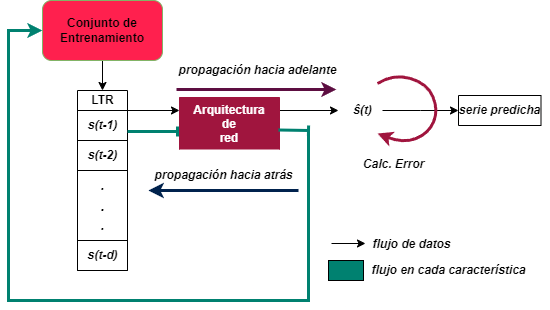
\includegraphics[width=0.8\textwidth]{Figuras/proceso_de_entrenamiento/Reforzamiento_del_profesor.png}
    \caption{Diagrama del reforzamiento del profesor.} 
    \label{fig:reforzamiento_profesor}
\end{figure}

\newpage
%%%%%%%%%%%%%%%%%%%%%%%%%%%%%%%%%%%%%%%%%
\subsection{NARNN}

Cuando todas las características del lote cuentan con su correspondiente predicción es cuando LM ejecuta un paso, modificando los pesos y sesgos de la red a partir del gradiente y matriz hessiana de la función de error.

Para encontrar el conjunto adecuado de hiper-parámetros para la fase de optimización, se analizó la combinación de la tasa de aprendizaje contra el número de épocas, manteniendo un tamaño de lote de uno. Comenzamos arbitrariamente en cualquier punto de la tabla, y se direcciona la búsqueda hacia donde el error en cada época parezca disminuir lo suficiente.

\begin{figure}[H]
    \centering
    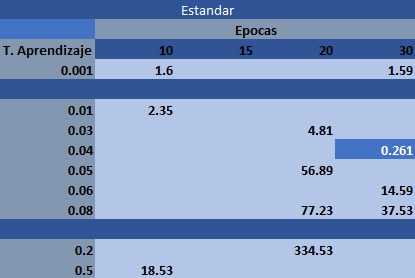
\includegraphics[width=0.7\textwidth]{Figuras/proceso_de_entrenamiento/lr_epocas_NARNN_estandar.png}
    \caption{Tabla comparativa entre combinaciones de parámetros de la NARNN: tasa de aprendizaje contra número épocas} 
    \label{fig:lr_epocas_NARNN}
\end{figure}

Como vemos, la mejor intersección se da en [0.04,30]. Para ilustrar que tan bien logrado es el entrenamiento a priori, se obtuvieron las siguientes predicciones sobre el mismo conjunto de entrenamiento en ambos tipos muestreos:

\begin{figure}[H]
    \begin{minipage}{0.5\textwidth}
        \centering
        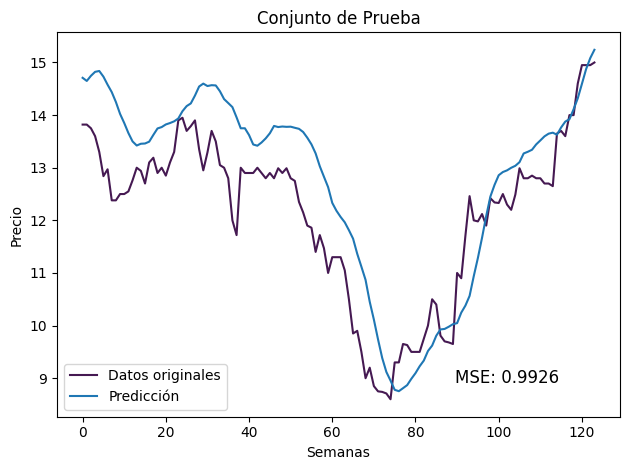
\includegraphics[width=\linewidth]{Figuras/proceso_de_entrenamiento/grafs_c_prueba/muestreo_aleatorio/NARNN/estandar/NARNN.png}
    \end{minipage}
    \begin{minipage}{0.5\textwidth}
        \centering
        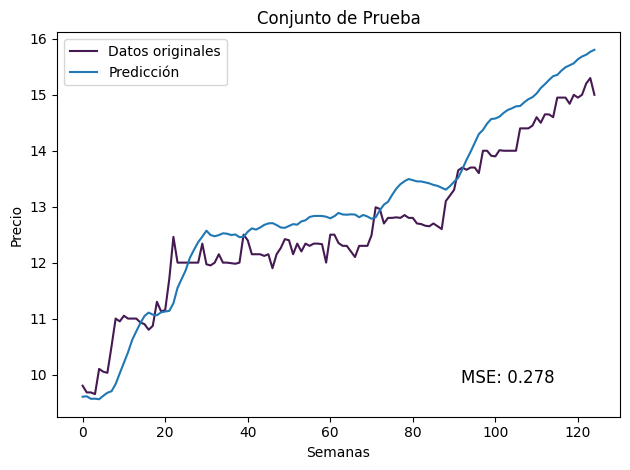
\includegraphics[width=\linewidth]{Figuras/proceso_de_entrenamiento/grafs_c_prueba/NARNN/estandar/NARNN.png}
        
    \end{minipage}
    \caption{Desempeño de la NARNN en conjunto de prueba: Muestro aleatorio y temporal} 
    \label{fig:c_prueba_NARNN}
\end{figure}

Cabe mencionar que encontrar los parámetros adecuados depende directamente de como estén inicializados estos. En general, para tanto la NARNN y la DWT-NARNN y para la longitud de datos de estudio representa un reto importante a la hora de encontrarlos \footnote{Como se ve reflejado en la tabla, el número de intentos en comparación a los de las RNNs es mayor}. 

En general las predicciones de NARNN son bastante aceptables, captando la dirección y comportamiento de la serie. Sin embargo, falla en captar los elementos 'sorpresivos' a los que este tipo de datos se atienen, como es el caso de los numerosos picos y hendiduras del muestreo temporal de las semanas veinte a ochenta.

\newpage

\subsection{DWT-NARNN}
Se procedió de manera similar que la NARNN, con la diferencia que se encontraron diferentes combinaciones de parámetros para las redes dedicadas a los componentes de detalle y de aproximación.

\begin{figure}[H]
    \centering
    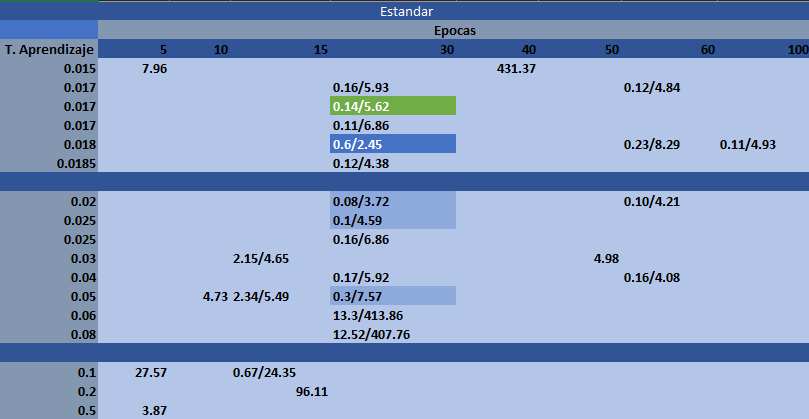
\includegraphics[width=0.7\textwidth]{Figuras/proceso_de_entrenamiento/lr_epocas_DWT_NARNN_estandar.png}
    \caption{Tabla comparativa entre combinaciones de parámetros de la DWT-NARNN: tasa de aprendizaje contra número épocas. (Los datos resaltados en verde representan la mejor combinaciones para las componentes de alta frecuencia y azul para los de baja).} 
    \label{fig:lr_epocas_DWTNARNN}
\end{figure}

\begin{figure}[H]
    \centering
    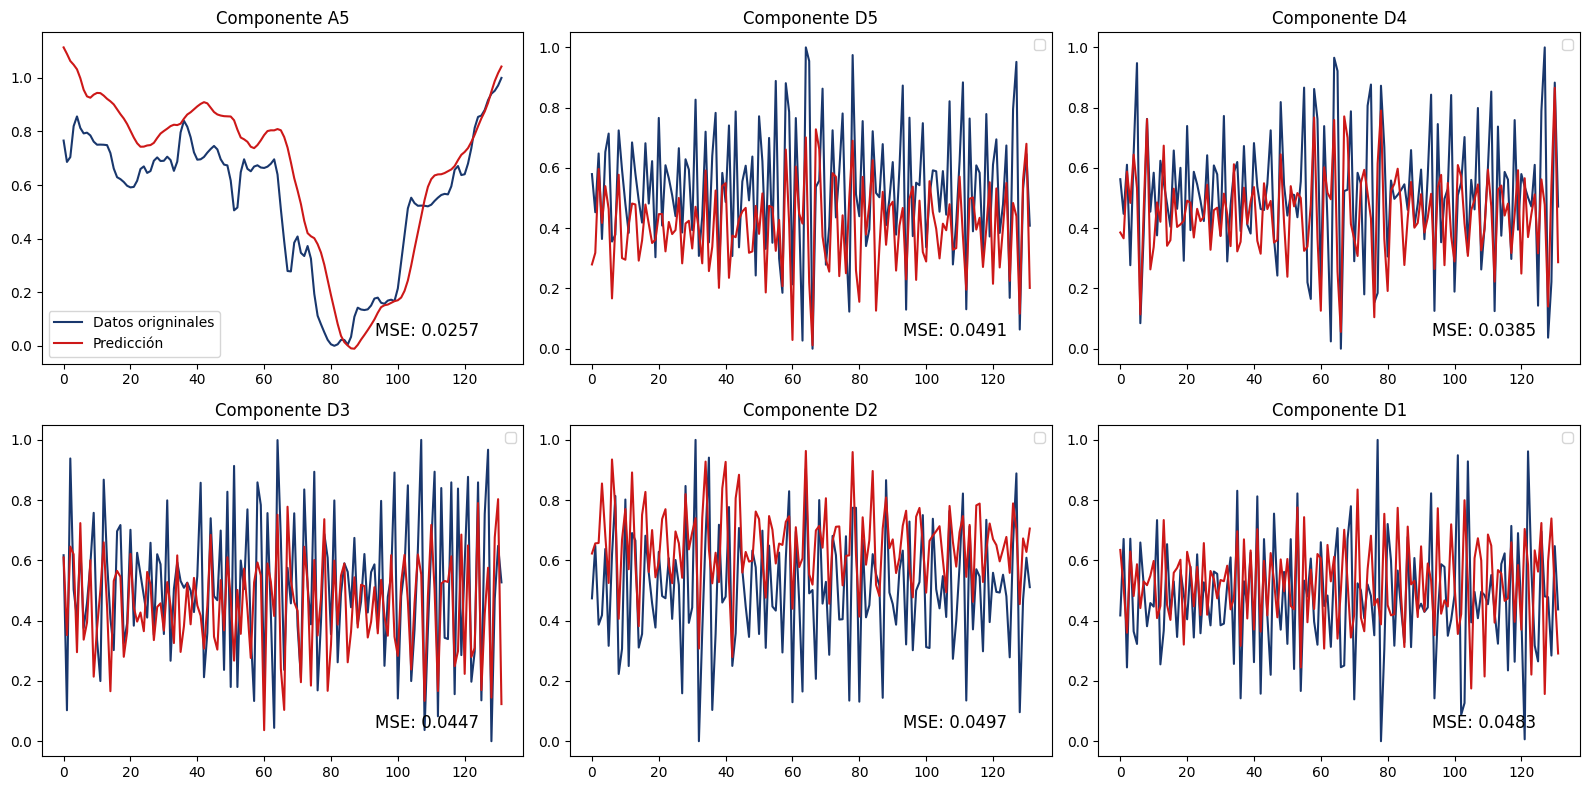
\includegraphics[width=0.9\textwidth]{Figuras/proceso_de_entrenamiento/grafs_c_prueba/muestreo_aleatorio/DWT_NARNN/estandar/DWT_NARNN.png}
    \caption{Predicciones de la DWT-LSTMnn de los componentes del conjunto de pruebas de muestro aleatorio.} 
    \label{fig:c_prueba_componentes_DWT_NARNN_aleatorio}
\end{figure}

\begin{figure}[H]
    \centering
    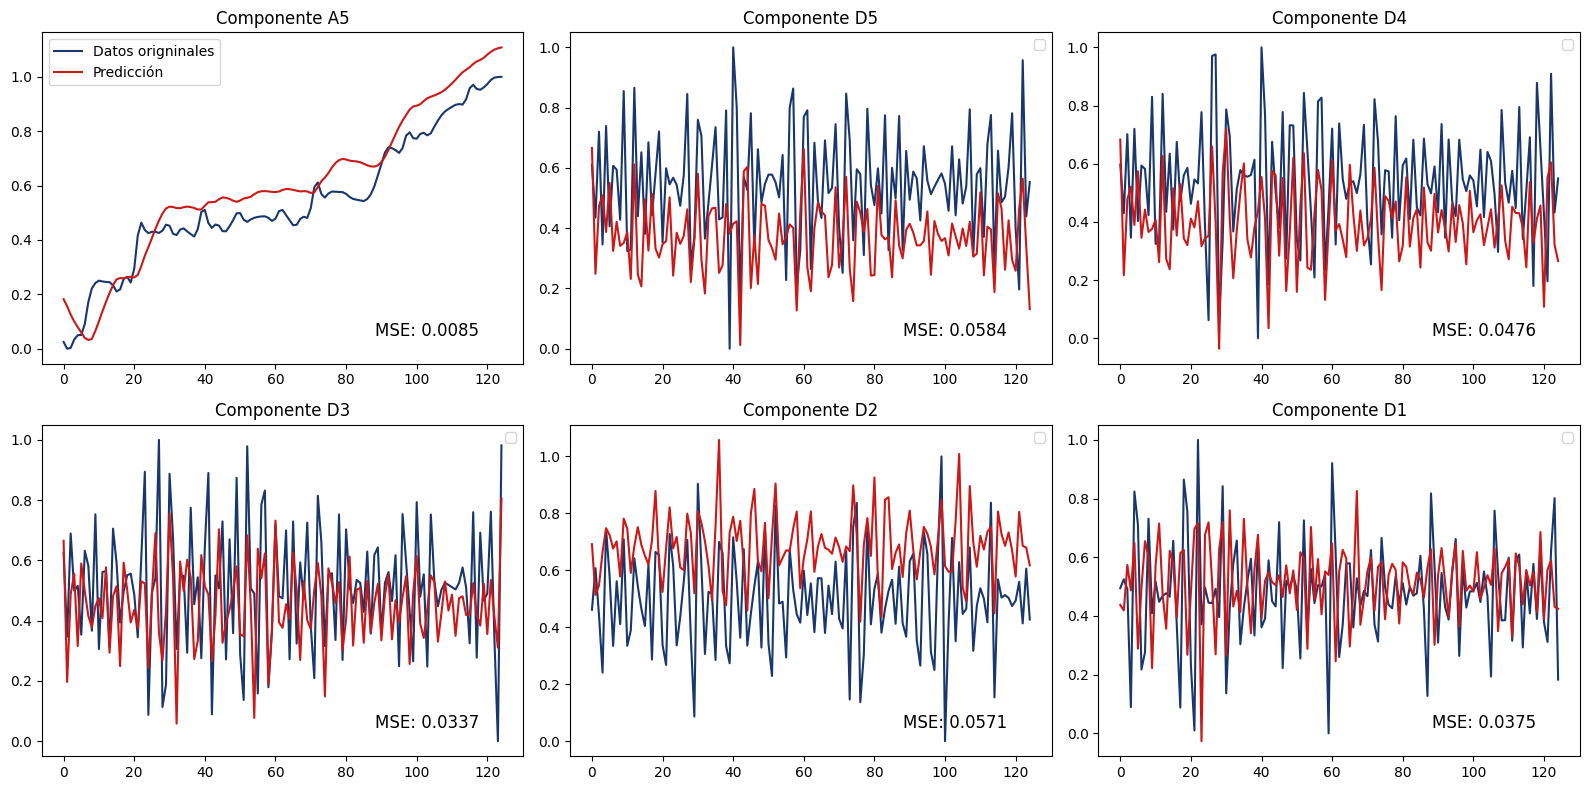
\includegraphics[width=0.9\textwidth]{Figuras/proceso_de_entrenamiento/grafs_c_prueba/DWT_NARNN/estandar/DWT_NARNN.png}
    \caption{Predicciones de la DWT-LSTMnn de los componentes del conjunto de pruebas de muestro temporal.} 
    \label{fig:c_prueba_componentes_DWT_NARNN}
\end{figure}

\begin{figure}[H]
    \begin{minipage}{0.5\textwidth}
        \centering
        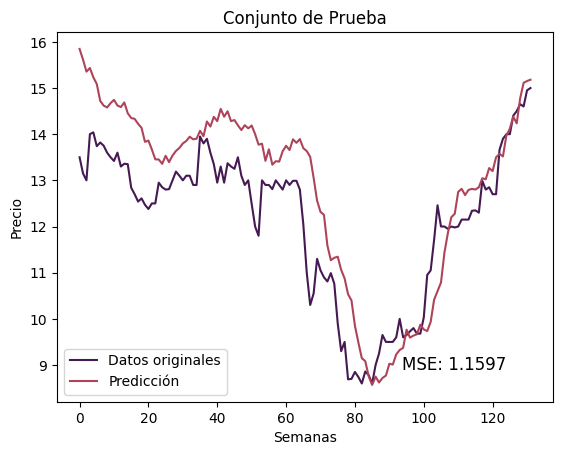
\includegraphics[width=\linewidth]{Figuras/proceso_de_entrenamiento/grafs_c_prueba/muestreo_aleatorio/DWT_NARNN/estandar/DWT_NARNN_rec.png}
    \end{minipage}
    \begin{minipage}{0.5\textwidth}
        \centering
        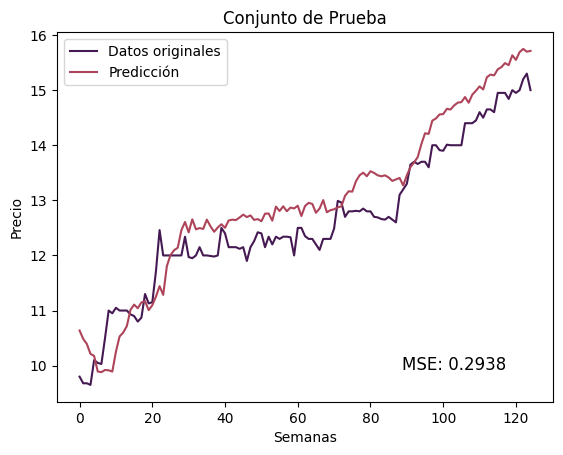
\includegraphics[width=\linewidth]{Figuras/proceso_de_entrenamiento/grafs_c_prueba/DWT_NARNN/estandar/DWT_NARNN_rec.png}
    \end{minipage}
    \caption{Desempeño de la DWT-NARNN en la reconstrucción del conjunto de prueba: Muestreo aleatorio y temporal.} 
    \label{fig:c_prueba_DWTNARNN}
\end{figure}

Se ve una notable mejoría en la captación de cambios subitos en las tendencias con respecto al modelo anterior, pero un aumento legero del error precisamente a estos cambios.

\newpage
%%%%%%%%%%%%%%%%%%%%%%%%%%%%%%%%%%%%%%%%%%%%%%%%%%%%%%%
\subsection{LSTMnn}

Encontrar los parámetros ideales en este caso empleó un menor esfuerzo. Partiendo de los datos que nos proporciona Adusumilli, Roshan, una tasa de aprendizaje de 0.0001, un tamaño de lote de 32 y 60 épocas, se obtuvieron muy buenos resultados en ambos muestreos:

\begin{figure}[H]
    \begin{minipage}{0.5\textwidth}
        \centering
        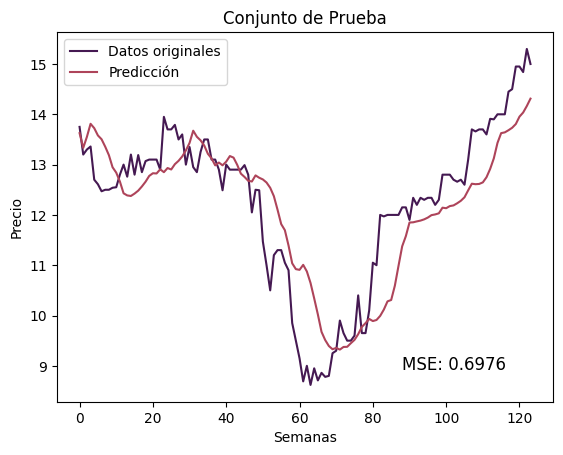
\includegraphics[width=\linewidth]{Figuras/proceso_de_entrenamiento/grafs_c_prueba/muestreo_aleatorio/LSTM/estandar/LSTM.png}
    \end{minipage}
    \begin{minipage}{0.5\textwidth}
        \centering
        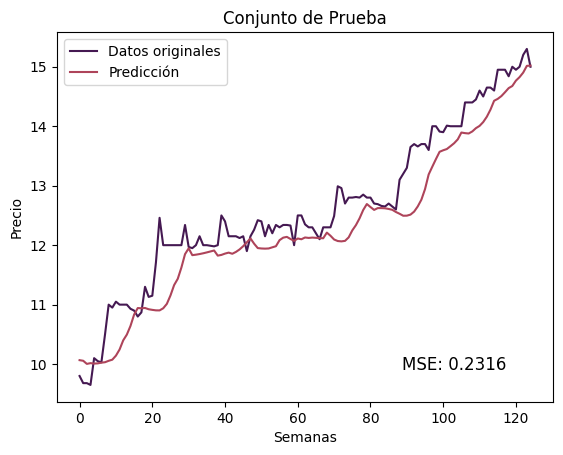
\includegraphics[width=\linewidth]{Figuras/proceso_de_entrenamiento/grafs_c_prueba/LSTM/estandar/LSTM.png}
    \end{minipage}
    \caption{Desempeño de la LSTMnn en conjunto de prueba: Muestreo aleatorio y temporal.} 
    \label{fig:c_prueba_LSTM}
\end{figure}

En comparación con los anteriores, mejora respecto a NARNN, pero sigue mostrando un poco de resistencia en ante cambios inesperados.

\newpage
%%%%%%%%%%%%%%%%%%%%%%%%%%%%%%%%%%%%%%%%%%%%%%%%%%%%%%%
\subsection{DWT-LSTMnn}

Se usaron los mismos parámetros que para la LSTMnn en la predicción de la componente \textit{A5} de baja frecuencia. Mientras que para las demás se procedió de manera similar a la NARNN y a la DWT-NARNN.

\begin{figure}[H]
    \centering
    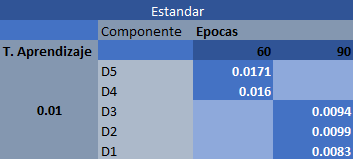
\includegraphics[width=0.5\textwidth]{Figuras/proceso_de_entrenamiento/lr_epocas_DWT_LSTM_estandar_componentes.png}
    \caption{Tabla comparativa entre parámetros para componentes de alta frecuencia de la DWT-LSTMnn: tasa de aprendizaje contra número épocas por cada componente.} 
    \label{fig:lr_epocas_DWT_LSTMnn_componentes}
\end{figure}

\begin{figure}[H]
    \centering
    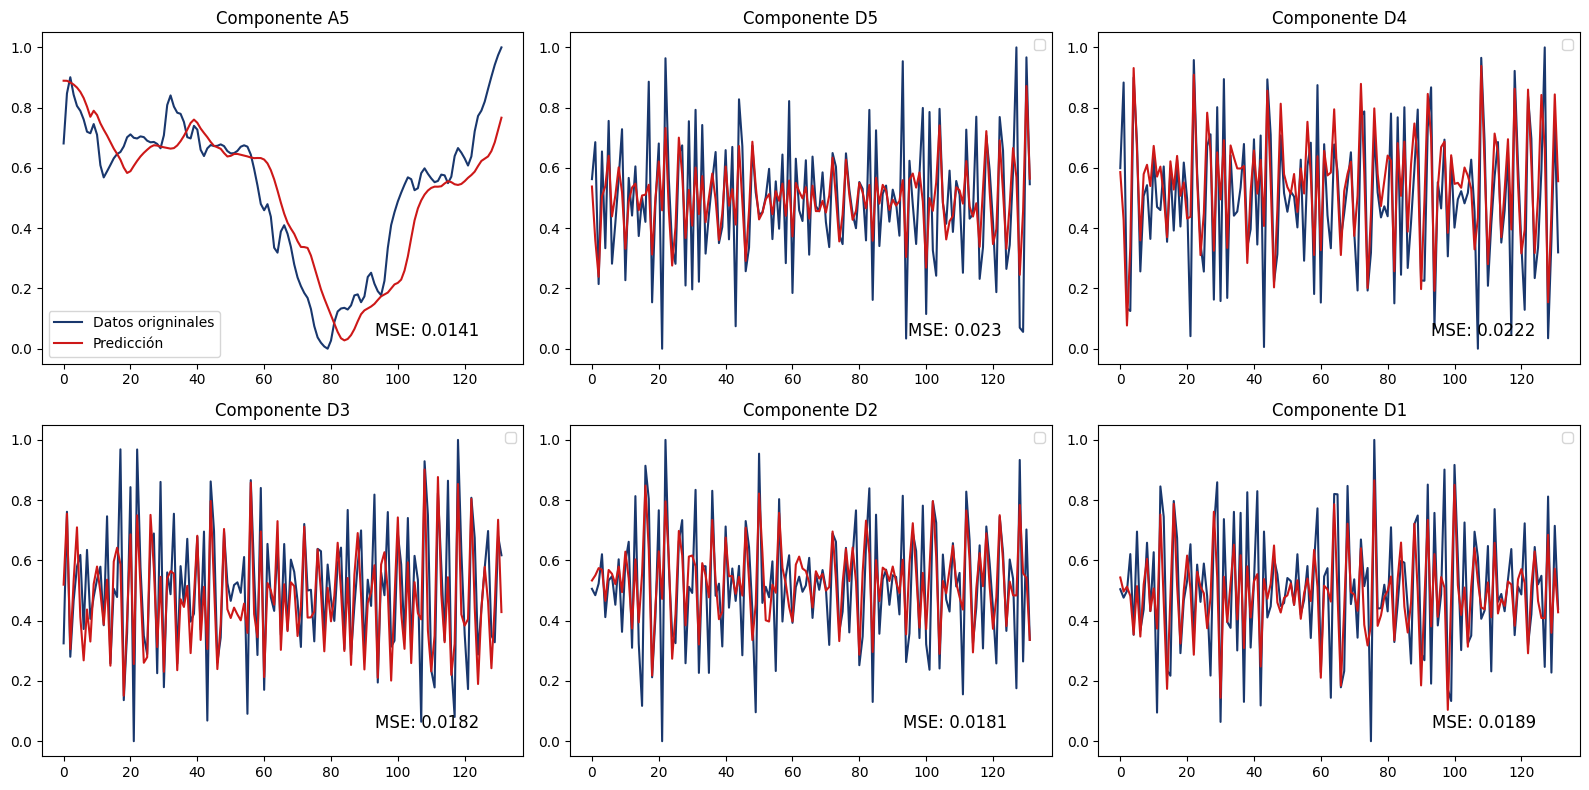
\includegraphics[width=0.9\textwidth]{Figuras/proceso_de_entrenamiento/grafs_c_prueba/muestreo_aleatorio/DWT_LSTM/estandar/DWT_LSTM.png}
    \caption{Predicciones de la DWT-LSTMnn de los componentes del conjunto de pruebas de muestro aleatorio.} 
    \label{fig:c_prueba_componentes_DWT_LSTM_aleatorio}
\end{figure}

\begin{figure}[H]
    \centering
    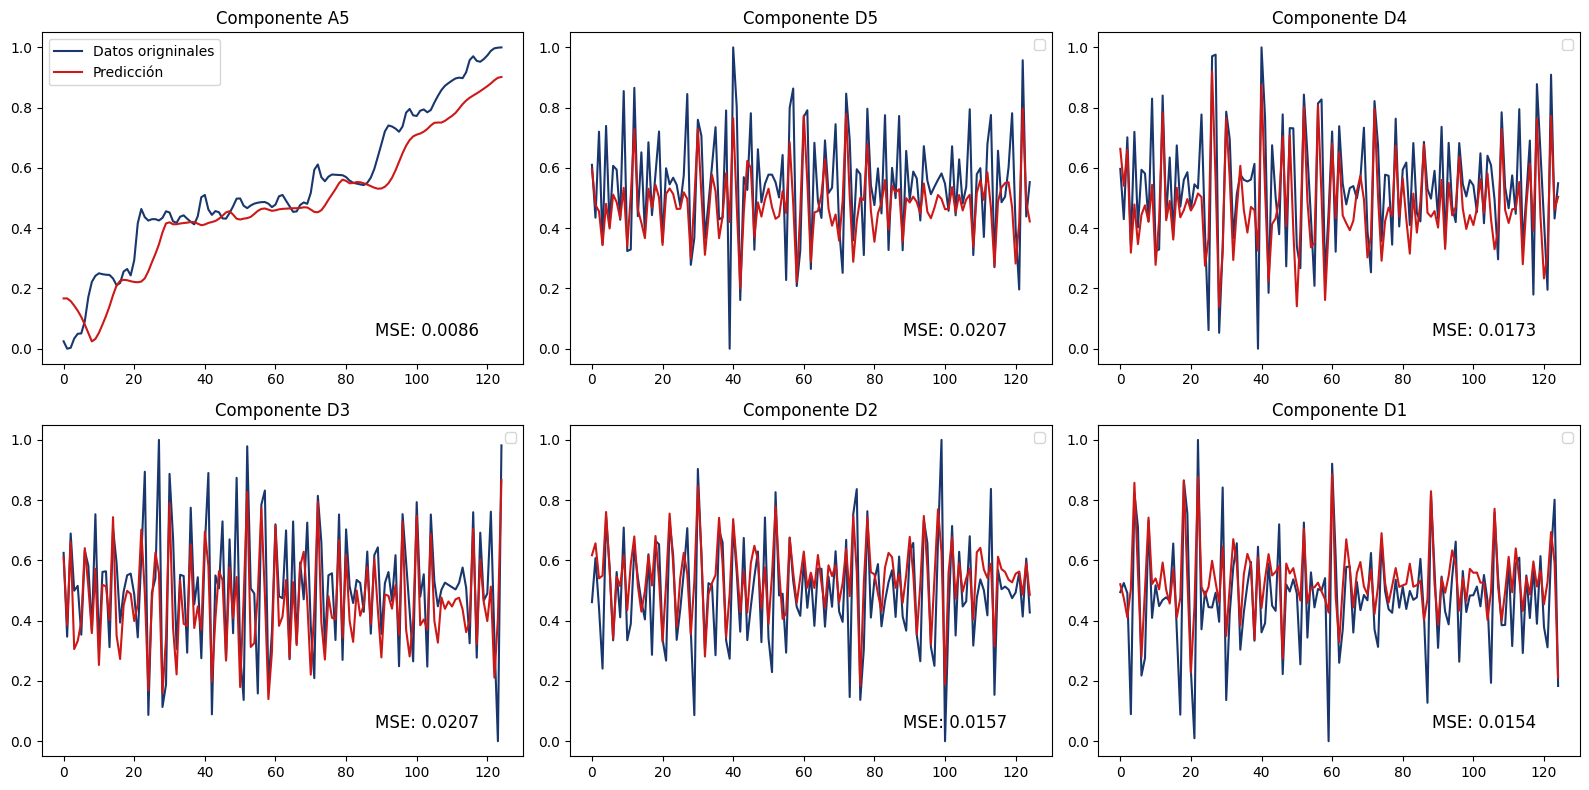
\includegraphics[width=0.9\textwidth]{Figuras/proceso_de_entrenamiento/grafs_c_prueba/DWT_LSTM/estandar/DWT_LSTM.png}
    \caption{Predicciones de la DWT-LSTMnn de los componentes del conjunto de pruebas de muestro temporal.} 
    \label{fig:c_prueba_componentes_DWT_LSTM}
\end{figure}

\begin{figure}[H]
    \begin{minipage}{0.5\textwidth}
        \centering
        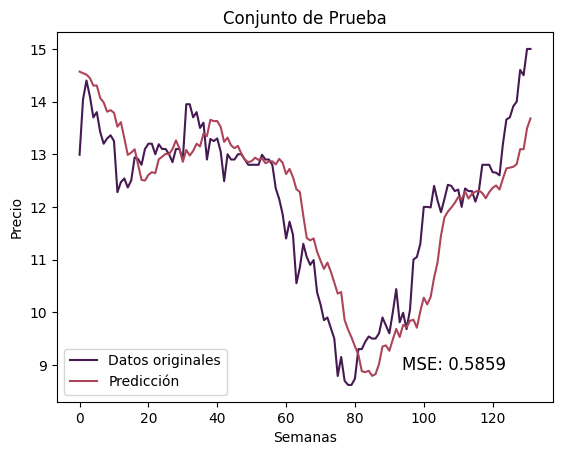
\includegraphics[width=\linewidth]{Figuras/proceso_de_entrenamiento/grafs_c_prueba/muestreo_aleatorio/DWT_LSTM/estandar/DWT_LSTM_rec.png}
    \end{minipage}
    \begin{minipage}{0.5\textwidth}
        \centering
        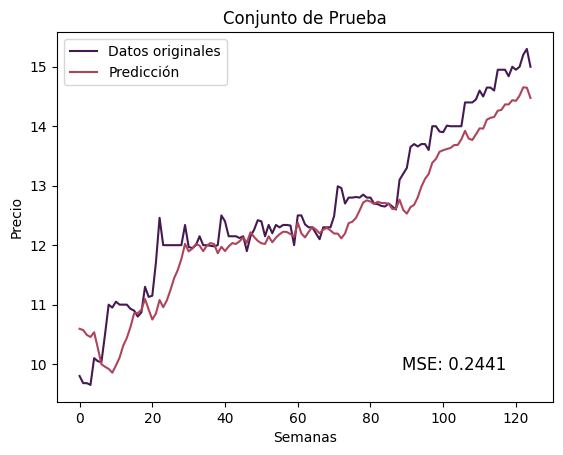
\includegraphics[width=\linewidth]{Figuras/proceso_de_entrenamiento/grafs_c_prueba/DWT_LSTM/estandar/DWT_LSTM_rec.png}
    \end{minipage}
    \caption{Desempeño de la DWT-LSTMnn en la reconstrucción del conjunto de prueba: Muestro aleatorio y temporal.} 
    \label{fig:c_prueba_DWTLSTM}
\end{figure}

Es clara la diferencia con DWT-NARNN, pues el error disminuye, y sigue manteniendo la capacidad de captar el 'ruido' de los datos. En ambos muestreos existen ventanas temporales donde la predicción se acerca bastante a los valores reales. Tal es el caso de las semanas treinta a sesenta del segundo ejemplo, posiblemente debido a el comportamiento en esos puntos.

\newpage
%%%%%%%%%%%%%%%%%%%%%%%%%%%%%%%%%%%%%%%%%%%%%%%%%%%%%%%
\subsection{GRUnn}

Al poseer una arquitectura paralela a las LSTMnn y la DWT-GRUnn a la DWT-LSTMnn, se hicieron uso de los mismos datos de entrenamiento. Obteniendo así:

\begin{figure}[H]
    \begin{minipage}{0.5\textwidth}
        \centering
        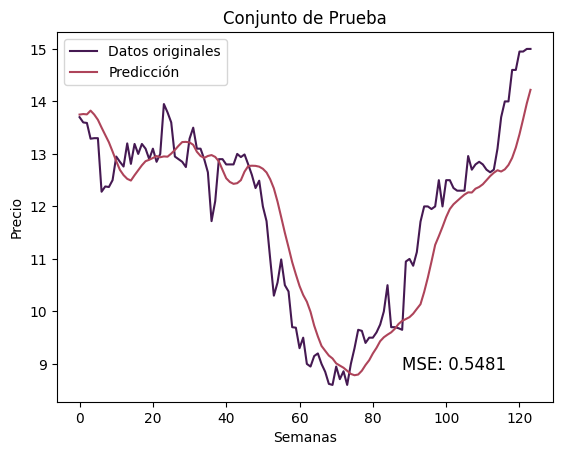
\includegraphics[width=\linewidth]{Figuras/proceso_de_entrenamiento/grafs_c_prueba/muestreo_aleatorio/GRU/estandar/GRU.png}
    \end{minipage}
    \begin{minipage}{0.5\textwidth}
        \centering
        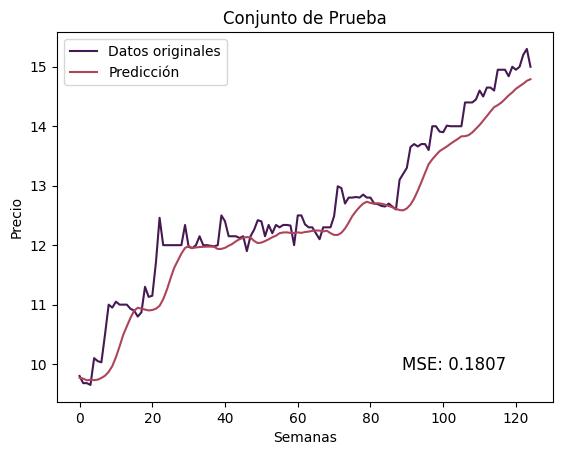
\includegraphics[width=\linewidth]{Figuras/proceso_de_entrenamiento/grafs_c_prueba/GRU/estandar/GRU.png}
    \end{minipage}
    \caption{Desempeño de la GRUnn en conjunto de prueba: Muestro aleatorio y temporal} 
    \label{fig:c_prueba_GRU}
\end{figure}

\newpage
%%%%%%%%%%%%%%%%%%%%%%%%%%%%%%%%%%%%%%%%%%%%%%%%%%%%%%%
\subsection{DWT-GRUnn}

\begin{figure}[H]
    \centering
    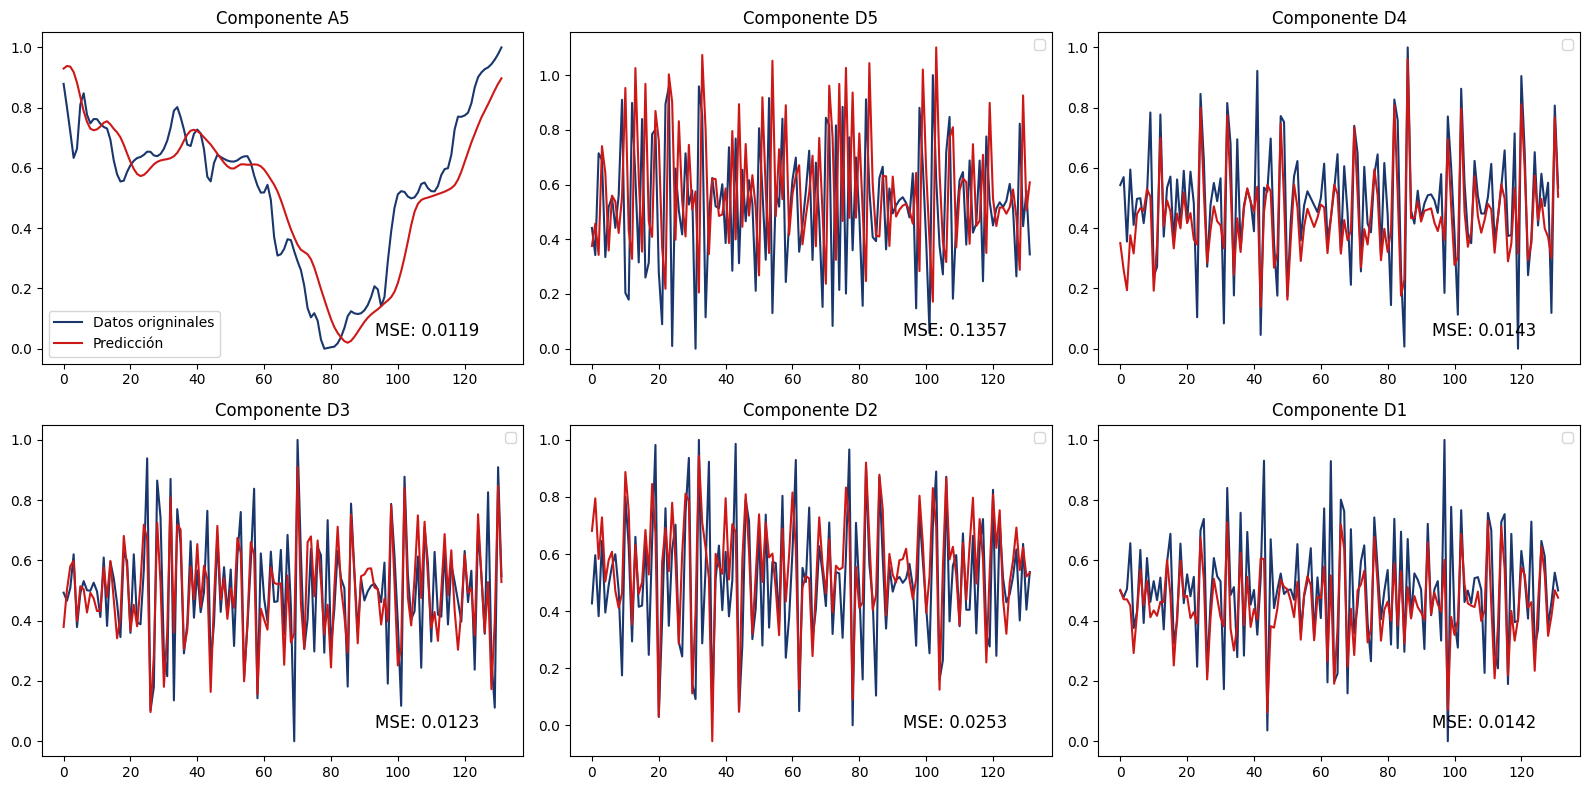
\includegraphics[width=0.9\textwidth]{Figuras/proceso_de_entrenamiento/grafs_c_prueba/muestreo_aleatorio/DWT_GRU/estandar/DWT_GRU.png}
    \caption{Predicciones de la DWT-GRUnn de los componentes del conjunto de pruebas de muestro aleatorio} 
    \label{fig:c_prueba_componentes_DWT_GRU_aleatorio}
\end{figure}

\begin{figure}[H]
    \centering
    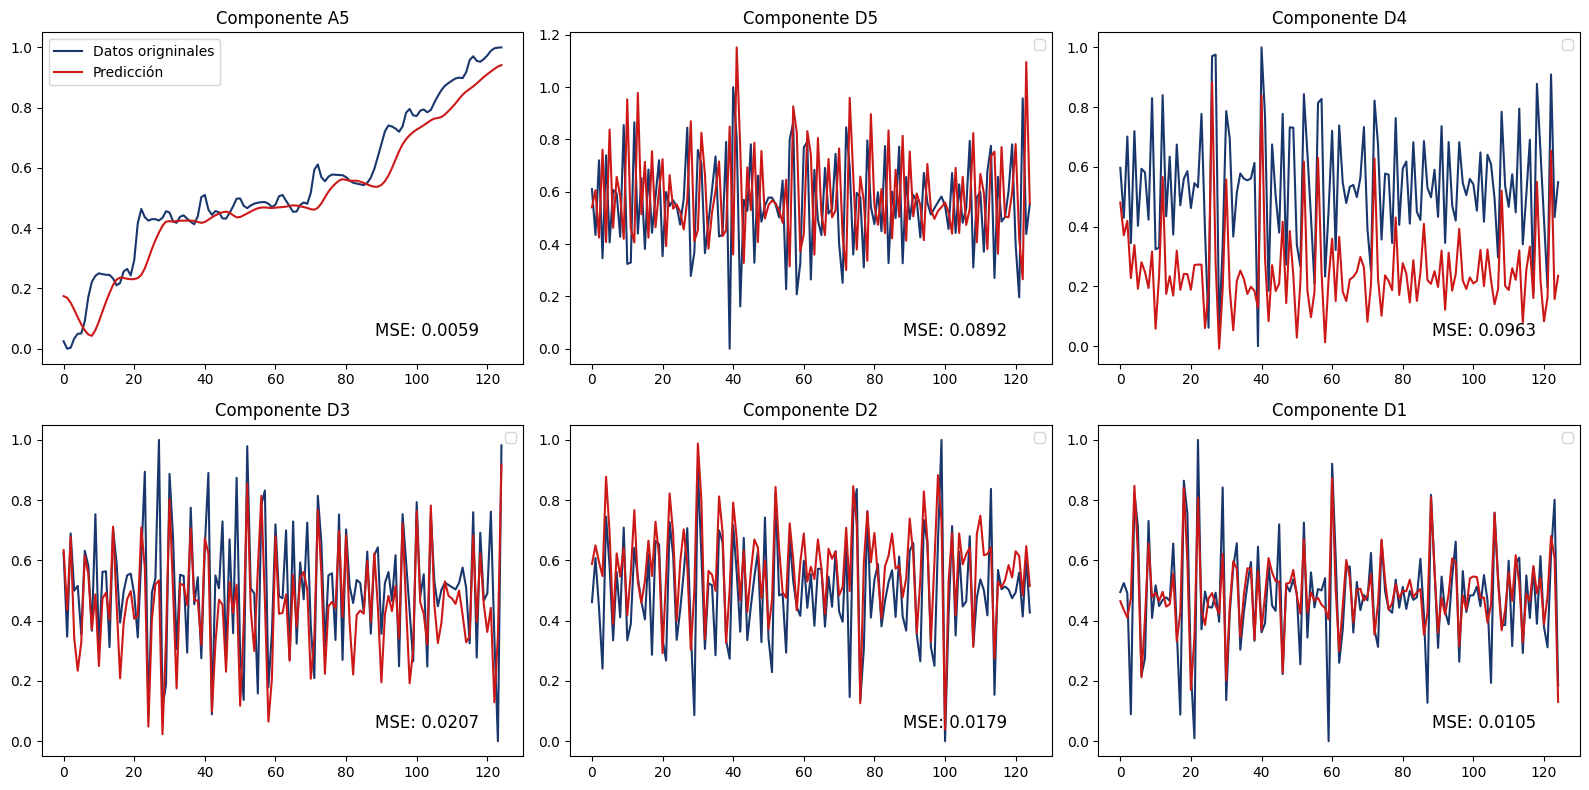
\includegraphics[width=0.9\textwidth]{Figuras/proceso_de_entrenamiento/grafs_c_prueba/DWT_GRU/estandar/DWT_GRU.png}
    \caption{Predicciones de la DWT-GRUnn de los componentes del conjunto de pruebas de muestro temporal} 
    \label{fig:c_prueba_componentes_DWT_GRU}
\end{figure}

Finalmente, y como ha ocurrido para los demás modelos que parten de redes recurrentes, se tomaron los mismos hiper-parametros para el DWT-GRUnn y se obtiene lo mostrado en las figuras \ref{fig:c_prueba_componentes_DWT_GRU_aleatorio} y \ref{fig:c_prueba_componentes_DWT_GRU}.

\begin{figure}[H]
    \begin{minipage}{0.5\textwidth}
        \centering
        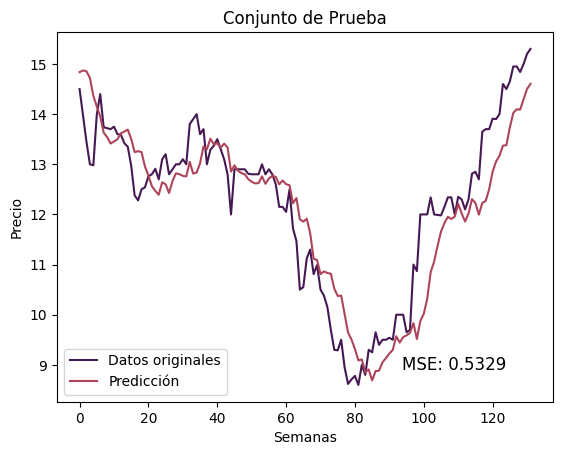
\includegraphics[width=\linewidth]{Figuras/proceso_de_entrenamiento/grafs_c_prueba/muestreo_aleatorio/DWT_GRU/estandar/DWT_GRU_rec.png}
    \end{minipage}
    \begin{minipage}{0.5\textwidth}
        \centering
        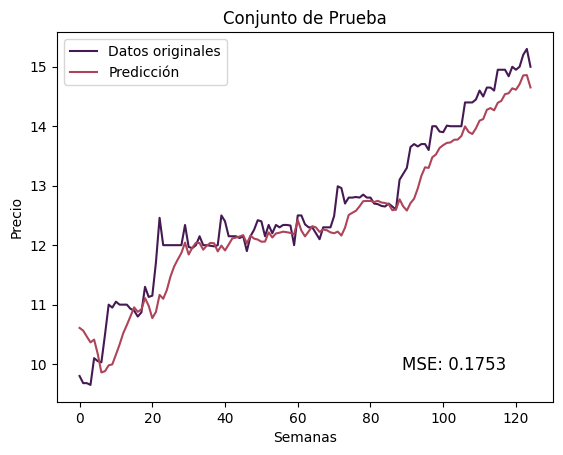
\includegraphics[width=\linewidth]{Figuras/proceso_de_entrenamiento/grafs_c_prueba/DWT_GRU/estandar/DWT_GRU_rec.png}
    \end{minipage}
    \caption{Desempeño de la DWT-GRUnn en la reconstrucción del conjunto de prueba: Muestro aleatorio y temporal.} 
    \label{fig:c_prueba_DWTGRU}
\end{figure}

Es bastante visible la mejoría que presenta la red GRU tanto en DWT-GRUnn como en GRUnn respecto a sus pares, en todas las predicciones el error disminuye y parece acercarse más a la serie original. Con o sin transformada de ondículas este enfoque de ANNs puede verse muy positivo para el pronostico de datos unidimensionales.

\newpage

\section{Entrenamiento Auto-predictivo}

De la misma manera que en la sección anterior, la entrada del conjunto de datos serán los precios de las primeras ocho semanas del conjunto de entrenamiento, para predecir el valor de la novena semana. Esa novena semana se concatenará como parte de la entrada en la predicción del precio siguiente semana, ocupando el lugar del octavo valor y repitiendo esto en las siguientes iteraciones. De esta forma, durante el cálculo de cada predicción se tomará como entrada a $[\hat{t}_{n-1}, \hat{t}_{n-2}, ..., \hat{t}_{n-8}]$ donde $\hat{t_i}$ es la predicción \textit{i-ésima} de la red, obteniendo $\hat{t_n}$. En la figura \ref{fig:entrenamiento_auto_predictivo} se puede ver en detalle la estructura de este enfoque.

\begin{figure}[h]
    \centering
    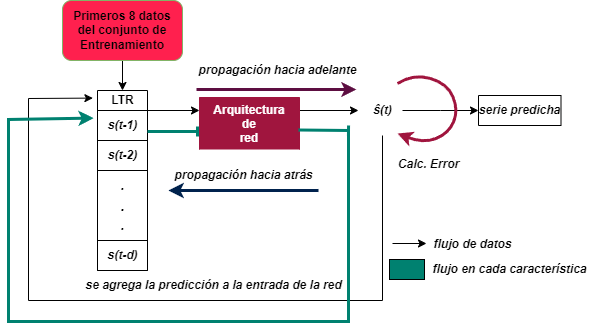
\includegraphics[width=0.8\textwidth]{Figuras/proceso_de_entrenamiento/Entrenamiento_auto_predictivo.png}
    \caption{Diagrama del entrenamiento auto-predictivo} 
    \label{fig:entrenamiento_auto_predictivo}
\end{figure}

Es importante recalcar que este experimento es de gran importancia para nuestro propósito, pues evaluará la autonomía de las redes para identificar tendencias de largo plazo. Sin embargo, no es el enfoque final del proyecto y se trata de un ambiente extremo al que se someten los modelos. Se toma un escenario para el cual el modelo solo dispone de ocho datos para predecir los consecuentes $n$ referentes al restante conjunto de datos. Con una información tan pequeña a disponer es imposible que se pueda mantener una predicción que pretenda ajustarse a un intervalo tan largo teniendo un punto de partida tan pequeño, pues el error que acarrea con las salidas predichas se acumula, y no es el objetivo predecir exactamente lo que sucederá, si no enfocarnos en cierta tendencia. Entonces, la finalidad de este análisis es puramente demostrativo, se busca encontrar qué modelo puede generar el mejor pronóstico en el peor escenario posible. 

%%%%%%%%%%%%%%%%%%%%%%%%%%%%%%%%%%%%%%%%%%%%%%%%%%%%%%%%%%%%%%%%%%%%%%
\subsection{NARNN}

La obtención de los hiper-parámetros de las redes ocurre de la misma manera analítica que en la subsección pasada. De esta forma, como se puede ver en la figura \ref{fig:lr_epocas_NARNN_autopred}, la mejor taza de aprendizaje y épocas son [0.0008,30].

\begin{figure}[H]
    \centering
    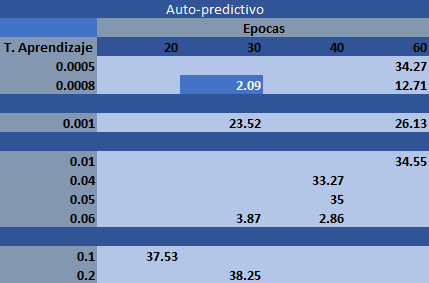
\includegraphics[width=0.5\textwidth]{Figuras/proceso_de_entrenamiento/lr_epocas_NARNN_auto_pred.png}
    \caption{Tabla comparativa entre parámetros de la NARNN: tasa de aprendizaje contra número épocas durante entrenamiento auto-predictivo.} 
    \label{fig:lr_epocas_NARNN_autopred}
\end{figure}

Con este entrenamiento, los pronósticos del conjunto de prueba son:

\begin{figure}[H]
    \begin{minipage}{0.5\textwidth}
        \centering
        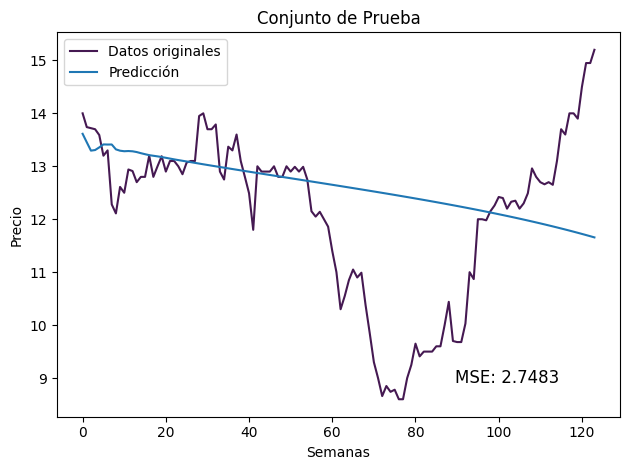
\includegraphics[width=\linewidth]{Figuras/proceso_de_entrenamiento/grafs_c_prueba/muestreo_aleatorio/NARNN/auto_predictiva/NARNN.png}
    \end{minipage}
    \begin{minipage}{0.5\textwidth}
        \centering
        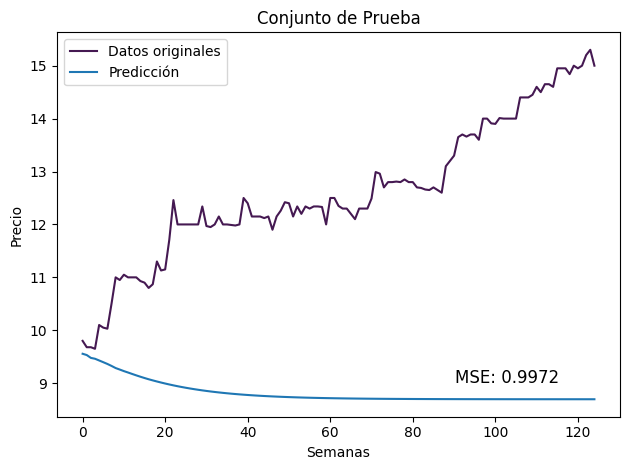
\includegraphics[width=\linewidth]{Figuras/proceso_de_entrenamiento/grafs_c_prueba/NARNN/auto_predictiva/NARNN.png}
    \end{minipage}
    \caption{Desempeño auto-predictivo de la NARNN en conjunto de prueba: Muestro aleatorio y temporal.} 
    \label{fig:c_prueba_NARNN_autopred_1}
\end{figure}

Vemos que en lo que respecta a la predicción, no encaja bien con los valores esperados. Esto surge desde que los primeros resultados de predicción arrastran consigo cierto error como se mencionaba más arriba y que, a la larga, este aumenta dándonos un resultado cada vez más inexacto. Por esta razón, se decidió agregar un nuevo parámetro, con el fin de estabilizar las primeras predicciones que la red nos da, de manera que los valores subsecuentes a estas se encuentren no tan alejadas al valor real.

Se empleó una técnica de decaimiento en la tasa de aprendizaje durante una época, de manera que en los lotes más próximos al inicio de la serie serán para los cuales la red aprenda mejor, garantizando que las predicciones en un inicio sean más acertadas y en consecuencia las siguientes arrastren una cantidad menor de error. \textit{El factor de decaimiento} (FD):

\begin{algorithm}[H]{
\caption{Ajuste del factor de decaimiento del aprendizaje}
\SetAlgoLined
\SetKwInOut{Input}{Entrada}
\SetKwInOut{Output}{Salida}

\SetKwFunction{onBatchBegin}{onBatchBegin}

%\Input{\textit{tasa actual}, \textit{lote}, \textit{tolerancia}, \textit{lote\_designado}}
%\Output{\textit{tasa actual}}

\BlankLine
\BlankLine

\SetKwProg{Fn}{alComenzarLote}{:}{}
    \Fn{(lote\_actual, perida\_actual)}{
        \BlankLine
            \If{perdida$\_$actual $\leq$ tolerancia \textbf{y} lote$\_$designado == lote$\_$actual}{
            factor$\_$de$\_$decaimiento = factor$\_$de$\_$decaimiento $\times$ 0.8\\
            %\tcp{Descomentar la siguiente línea si quieres imprimir el nuevo factor}
            %\tcp{print(f">>nuevo factor: {lr\_callback.decay\_factor}")}
            lote$\_$designado = lote$\_$designado + 1
            \BlankLine
            \tcp{El lote actual indica a partir de qué lote se empezará a tomar en cuenta el FD}
        }
        \BlankLine
        \textit{tasa\_actual}$ \gets \frac{\text{\textit{tasa\_inicial}}}{1 + \text{\textit{factor\_de\_decaimiento}} \times \text{\textit{iteracion}}}$ \tcp*{Calcula la nueva tasa de aprendizaje}
        \BlankLine
        %\textbf{Imprimir} "lr: ", lr, ", batch: ", batch \;
        \BlankLine
        \textit{iteracion}++ \tcp{Incrementa el número de iteración}
        %$\text{iteracion} \gets \text{iteracion} + 1$ \;
        \BlankLine
        \textbf{regresa} \textit{tasa\_actual} \;
    }
}
\end{algorithm}

Así, durante cada época si la pérdida actual es menor a la tolerancia y el lote designado es el actual, el FD cae, y la penalización de la tasa de aprendizaje en los siguientes lotes es menor. De cualquier forma se disminuye la tasa actual en función de la tasa inicial, el FD y el número de época o lote en el que nos encontramos.

Aplicando lo anterior, en la figura \ref{fig:lr_epocas_NARNN_autopred_v2} podemos ver un diagrama parecido a los anteriores, pero ahora considerando el FD como parte de la busqueda exahustiva de los hiper-parámetros.

\begin{figure}[H]
    \centering
    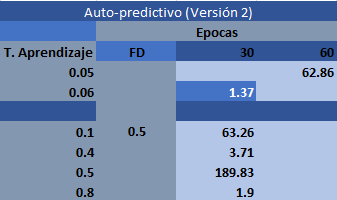
\includegraphics[width=0.5\textwidth]{Figuras/proceso_de_entrenamiento/lr_epocas_NARNN_auto_pred_v2.png}
    \caption{Tabla comparativa entre parámetros de la NARNN: tasa de aprendizaje contra número épocas y factor de decaimiento durante entrenamiento auto-predictivo.} 
    \label{fig:lr_epocas_NARNN_autopred_v2}
\end{figure}

\begin{figure}[h]
    \begin{minipage}{0.5\textwidth}
        \centering
        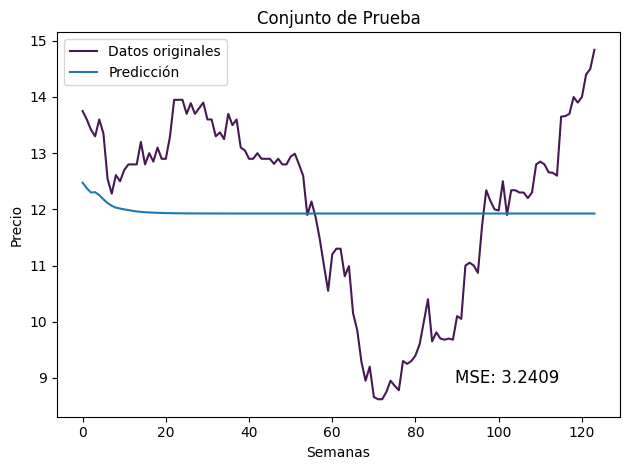
\includegraphics[width=\linewidth]{Figuras/proceso_de_entrenamiento/grafs_c_prueba/muestreo_aleatorio/NARNN/auto_predictiva/NARNN_v2.png}
    \end{minipage}
    \begin{minipage}{0.5\textwidth}
        \centering
        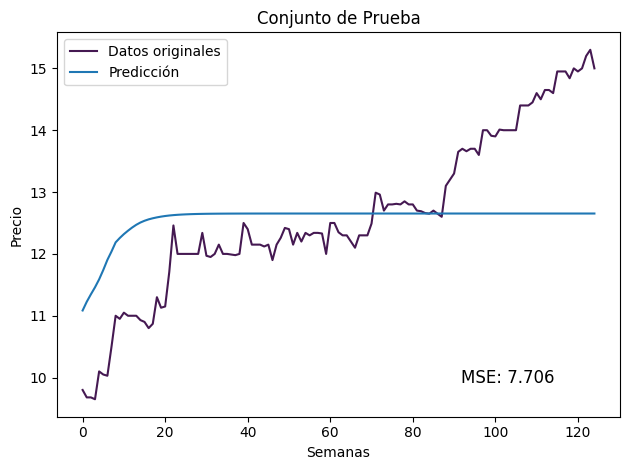
\includegraphics[width=\linewidth]{Figuras/proceso_de_entrenamiento/grafs_c_prueba/NARNN/auto_predictiva/NARNN_v2.png}
    \end{minipage}
    \caption{Desempeño auto-predictivo de la NARNN en conjunto de prueba bajo la implementación del factor de decaimiento: Muestro aleatorio y temporal.} 
    \label{fig:c_prueba_NARNN_autopred_v2}
\end{figure}

Encontrándonos así una mejor predicción en general \footnote{Notemos que esta técnica 'obliga' a la red a aprender mejor los primeros datos del conjunto en decremento de entendimiento que tiene de los subsecuentes. Hecho que perjudica a la predicción cualquier otro tipo de predicción que no sea enteramente auto-predictiva.}. Respecto al muestreo temporal, mejoró bastante, captando la tendencia creciente de los precios durante las primeras semanas, en contraposición de lo que se ve en el muestreo aleatorio que empeoro al inicio de las semanas.

%\newpage

%%%%%%%%%%%%%%%%%%%%%%%%%%%%%%%%%%%%%%%%%%%%%%%%%%%%%%%%%%%%%%%%%%%%%%
\subsection{DWT-NARNN}

En el mismo snetido, Se usaron los mismos parámetros que para la NARNN para el componente de baja frecuencia. Para los demás se encontró que un enfoque sin FD daba buen resultado.

\begin{figure}[H]
    \centering
    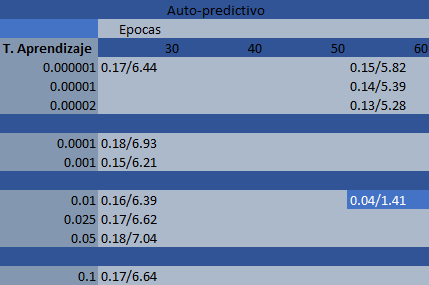
\includegraphics[width=0.5\textwidth]{Figuras/proceso_de_entrenamiento/lr_epocas_DWT_LSTM_auto_pred.png}
    \caption{Tabla comparativa entre parámetros de la DWT-NARNN para componentes de alta frecuencia: tasa de aprendizaje contra número épocas durante entrenamiento auto-predictivo.} 
    \label{fig:lr_epocas_DWTNARNN_autopred_v2}
\end{figure}

\begin{figure}[H]
    \centering
    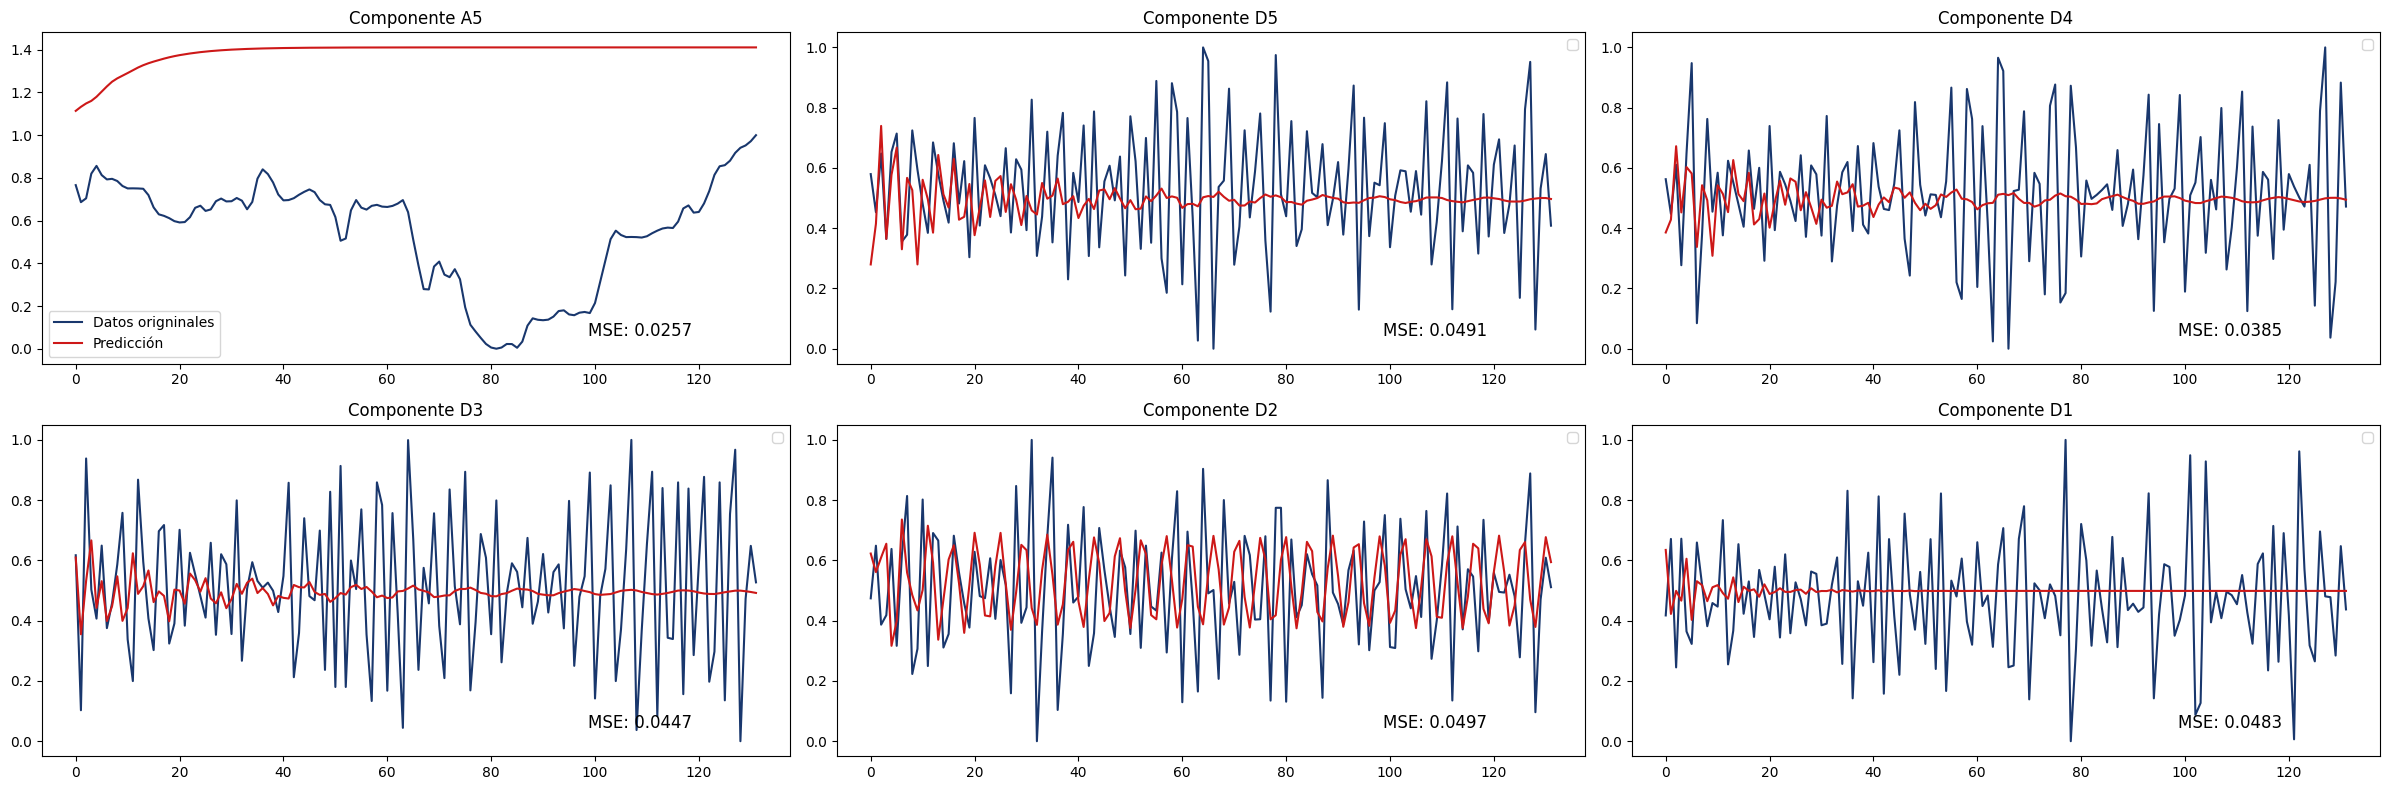
\includegraphics[width=0.9\textwidth]{Figuras/proceso_de_entrenamiento/grafs_c_prueba/muestreo_aleatorio/DWT_NARNN/auto_predictiva/DWT_NARNN.png}
    \caption{Predicciones auto-predictivas de la DWT-NARNNnn de los componentes del conjunto de pruebas de muestro aleatorio.} 
    \label{fig:c_prueba_componentes_DWTNARNN_autopred_aleatorio}
\end{figure}

\begin{figure}[H]
    \centering
    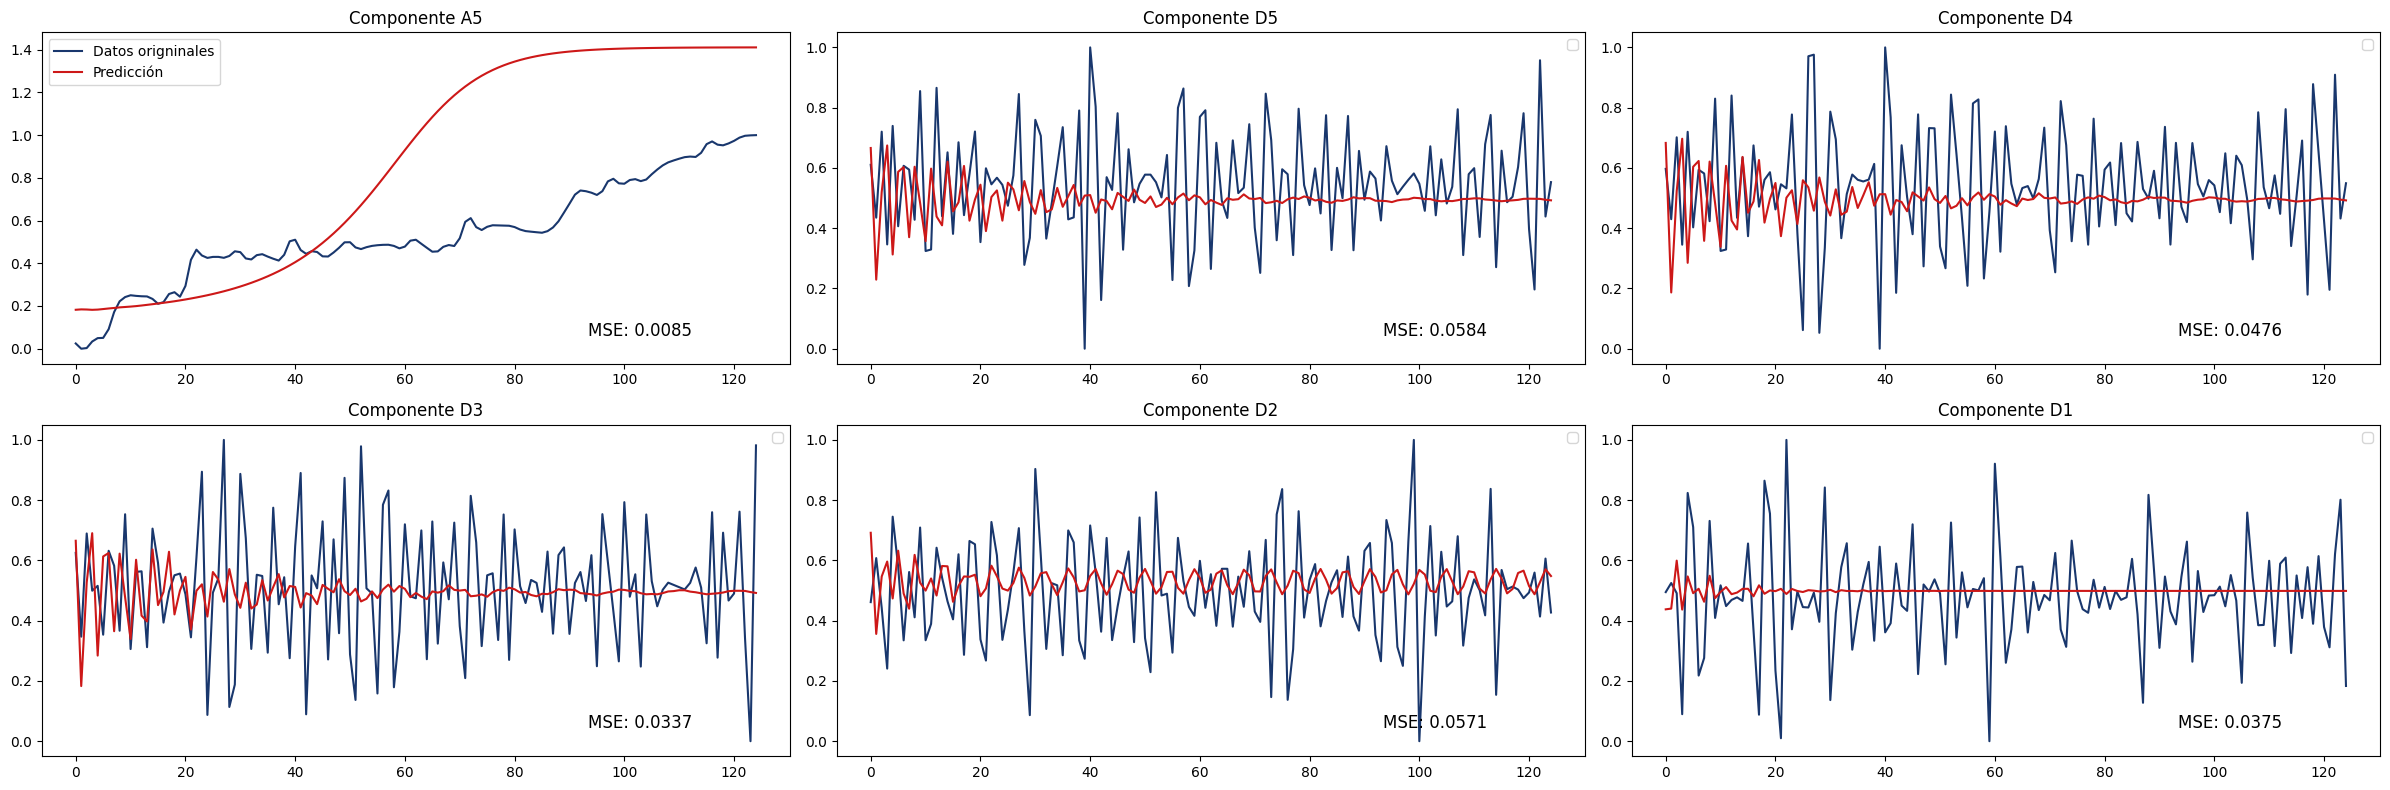
\includegraphics[width=0.9\textwidth]{Figuras/proceso_de_entrenamiento/grafs_c_prueba/DWT_NARNN/auto_predictiva/DWT_NARNN.png}
    \caption{Predicciones auto-predictivas de la DWT-NARNNnn de los componentes del conjunto de pruebas de muestro temporal.} 
    \label{fig:c_prueba_componentes_DWTNARNN_autopred}
\end{figure}

\begin{figure}[H]
    \begin{minipage}{0.5\textwidth}
        \centering
        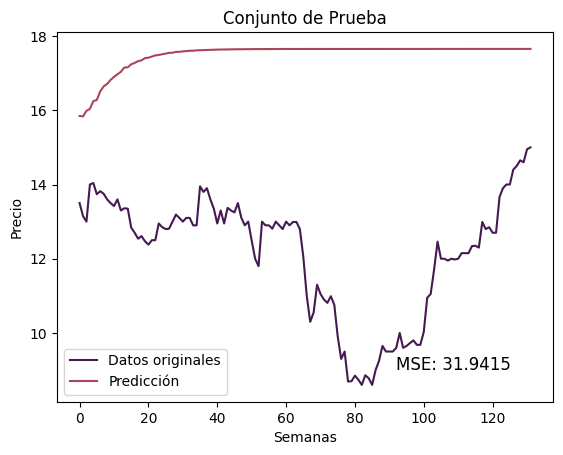
\includegraphics[width=\linewidth]{Figuras/proceso_de_entrenamiento/grafs_c_prueba/muestreo_aleatorio/DWT_NARNN/auto_predictiva/DWT_NARNN_rec.png}
    \end{minipage}
    \begin{minipage}{0.5\textwidth}
        \centering
        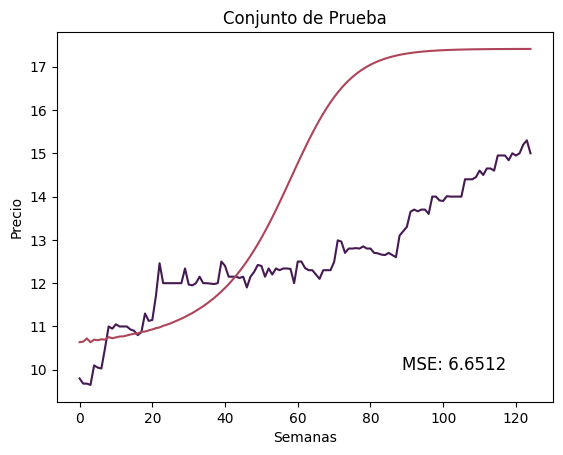
\includegraphics[width=\linewidth]{Figuras/proceso_de_entrenamiento/grafs_c_prueba/DWT_NARNN/auto_predictiva/DWT_NARNN_rec.png}
    \end{minipage}
    \caption{Desempeño auto-predictivo de la DWT-NARNNnn en conjunto de prueba: Muestro aleatorio y temporal.} 
    \label{fig:c_prueba_DWTNARNN_autopred_v2}
\end{figure}
%%%%%%%%%%%%%%%%%%%%%%%%%%%%%%%%%%%%%%%%%%%%%%%%%%%%%%%%%%%%%%%%%%%%%%
\newpage
\subsection{LSTMnn}

En el mismo sentido que la NARNN, los resultados del entrenamiento auto-predictivo sin implementar el factor de decaimiento no son muy alentadores.

\begin{figure}[H]
    \centering
    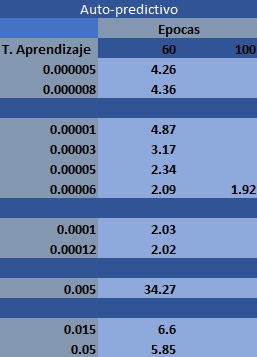
\includegraphics[width=0.45\textwidth]{Figuras/proceso_de_entrenamiento/lr_epocas_LSTM_auto_pred.png}
    \caption{Tabla comparativa entre parámetros de la LSTMnn: tasa de aprendizaje contra número épocas en un entrenamiento auto-predictivo.} 
    \label{fig:lr_epocas_LSTMnn_autopred}
\end{figure}

\newpage

Aplicando un estudio de la misma manera que la NARNN. Tenemos:

\begin{figure}[H]
    \centering
    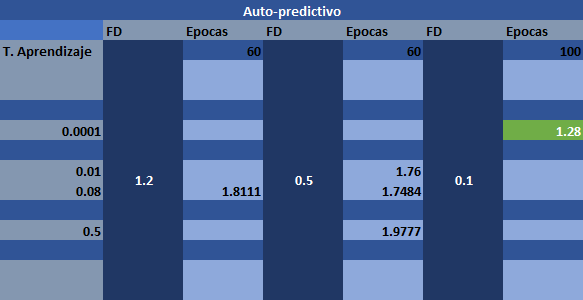
\includegraphics[width=0.8\textwidth]{Figuras/proceso_de_entrenamiento/lr_epocas_LSTM_autopred_v2.png}
    \caption{Tabla comparativa entre parámetros de la LSTMnn: tasa de aprendizaje contra número épocas en un entrenamiento auto-predictivo con factor de decaimiento.} 
    \label{fig:lr_epocas_LSTMnn_autopred_v2}
\end{figure}

\begin{figure}[H]
    \begin{minipage}{0.5\textwidth}
        \centering
        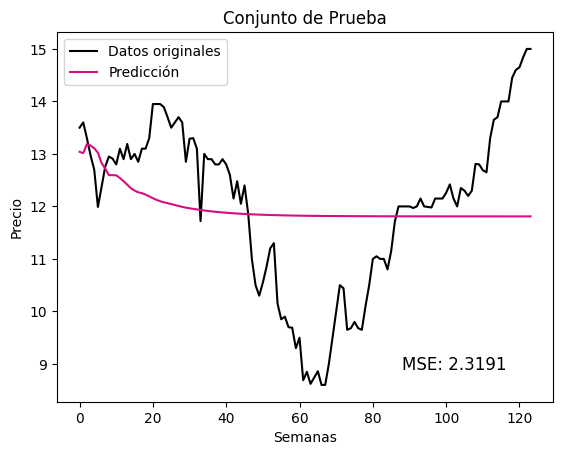
\includegraphics[width=\linewidth]{Figuras/proceso_de_entrenamiento/grafs_c_prueba/muestreo_aleatorio/LSTM/auto_predictiva/LSTM_v2.png}
    \end{minipage}
    \begin{minipage}{0.5\textwidth}
        \centering
        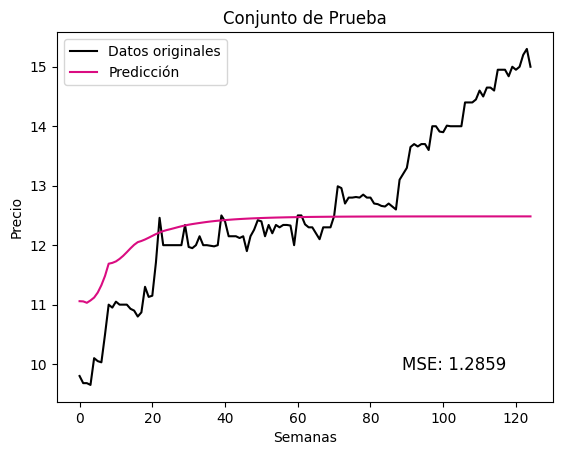
\includegraphics[width=\linewidth]{Figuras/proceso_de_entrenamiento/grafs_c_prueba/LSTM/auto_predictiva/LSTM_v2.png}
    \end{minipage}
    \caption{Desempeño auto-predictivo de la LSTMnn en conjunto de prueba: muestreo aleatorio y temporal.} 
    \label{fig:c_prueba_LSTM_autopred_v2}
\end{figure}

\newpage

\subsection{DWT-LSTMnn}

Para este entrenamiento, se obtuvieron los siguientes resultados. 

\begin{figure}[H]
    \centering
    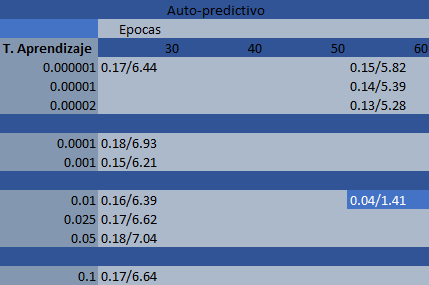
\includegraphics[width=0.6\textwidth]{Figuras/proceso_de_entrenamiento/lr_epocas_DWT_LSTM_auto_pred.png}
    \caption{Tabla comparativa entre parámetros de la DWT-LSTMnn: tasa de aprendizaje contra número épocas y factor de decaimiento durante entrenamiento auto-predictivo.} 
    \label{fig:lr_epocas_DWTLSTM_autopred_v2}
\end{figure}

Tomando la misma combinación de parámetros para las redes destinadas a cada componente.

\begin{figure}[H]
    \centering
    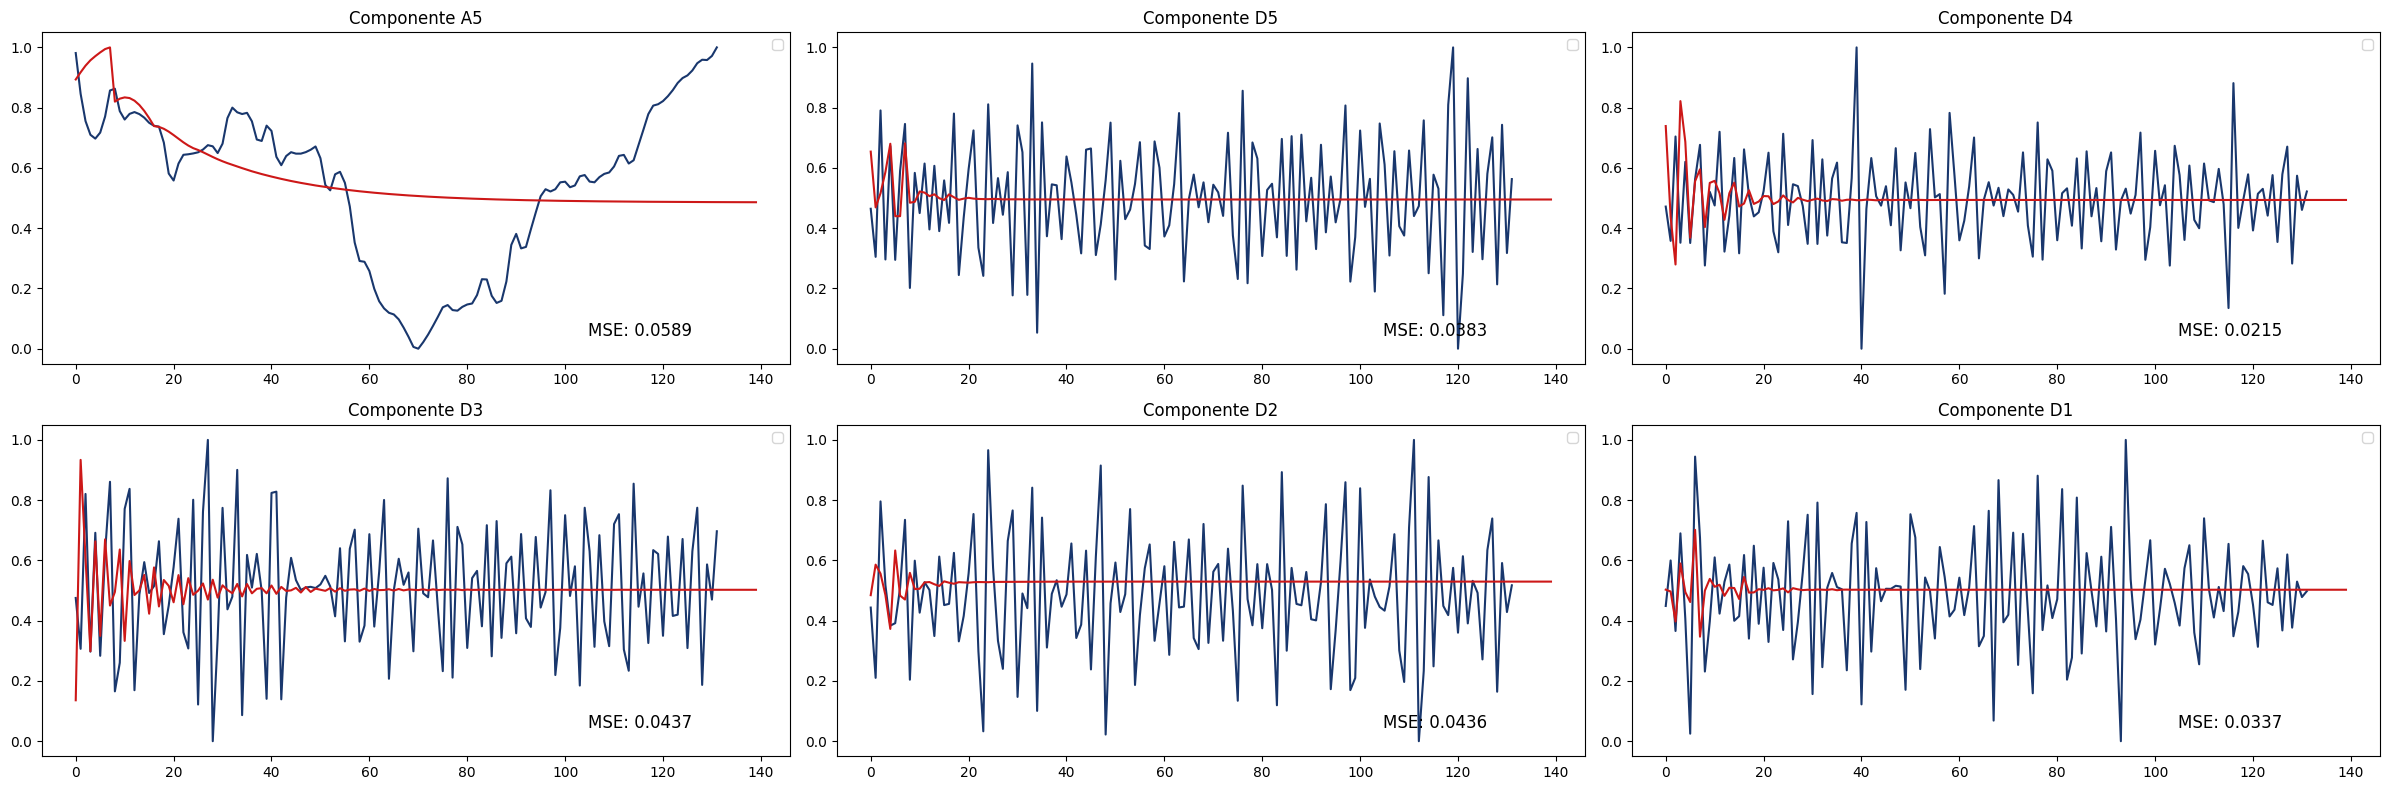
\includegraphics[width=0.9\textwidth]{Figuras/proceso_de_entrenamiento/grafs_c_prueba/muestreo_aleatorio/DWT_LSTM/auto_predictiva/DWT_LSTM.png}
    \caption{Predicciones auto-predictivas de la DWT-LSTMnn de los componentes del conjunto de pruebas de muestro aleatorio.} 
    \label{fig:c_prueba_componentes_DWTLSTM_autopred_aleatorio}
\end{figure}

\begin{figure}[H]
    \centering
    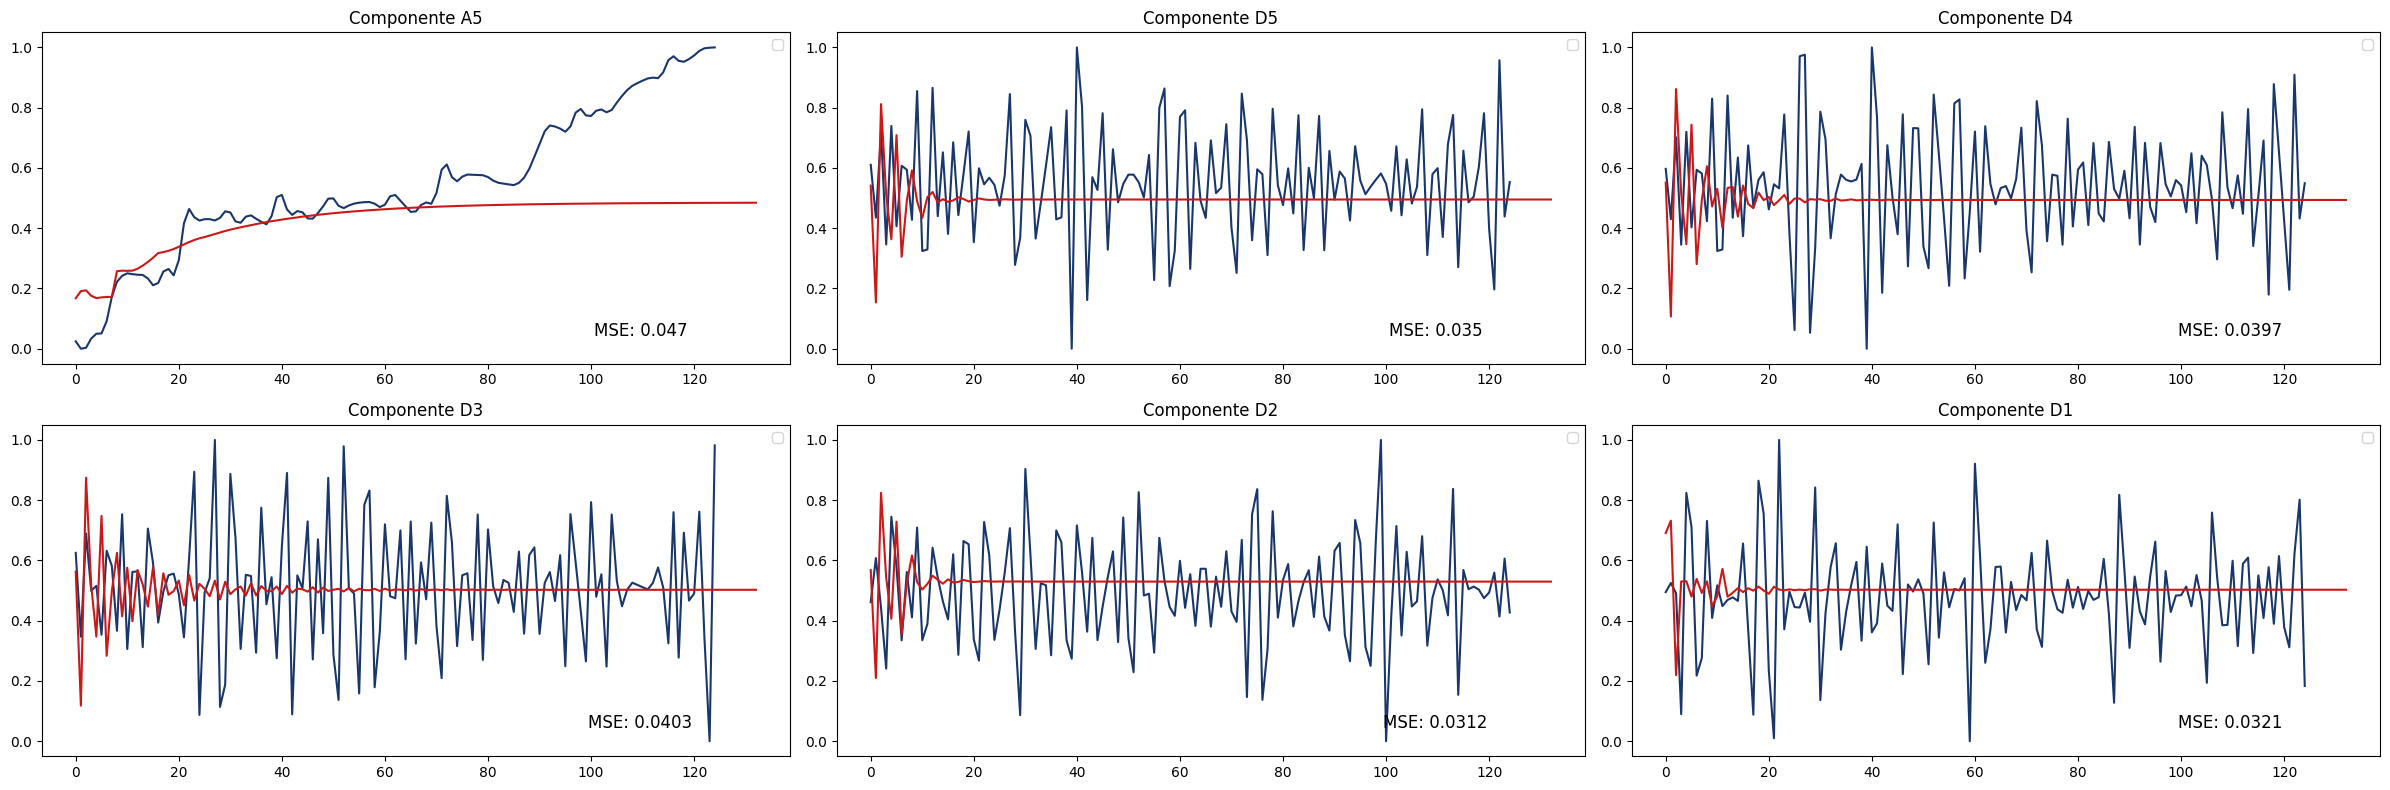
\includegraphics[width=0.9\textwidth]{Figuras/proceso_de_entrenamiento/grafs_c_prueba/DWT_LSTM/auto_predictiva/DWT_LSTM.png}
    \caption{Predicciones auto-predictivas de la DWT-LSTMnn de los componentes del conjunto de pruebas de muestro temporal.} 
    \label{fig:c_prueba_componentes_DWTLSTM_autopred}
\end{figure}

\begin{figure}[H]
    \begin{minipage}{0.5\textwidth}
        \centering
        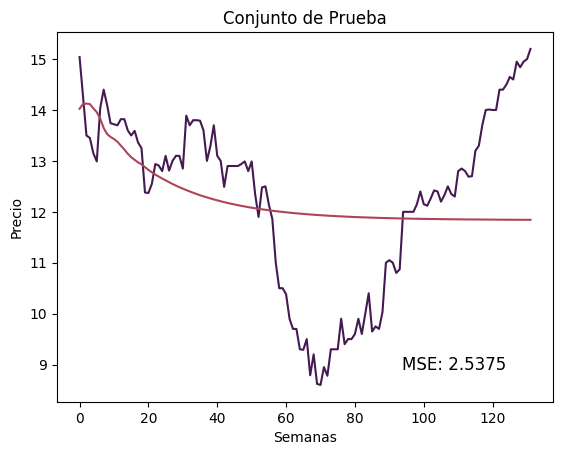
\includegraphics[width=\linewidth]{Figuras/proceso_de_entrenamiento/grafs_c_prueba/muestreo_aleatorio/DWT_LSTM/auto_predictiva/DWT_LSTM_rec.png}
    \end{minipage}
    \begin{minipage}{0.5\textwidth}
        \centering
        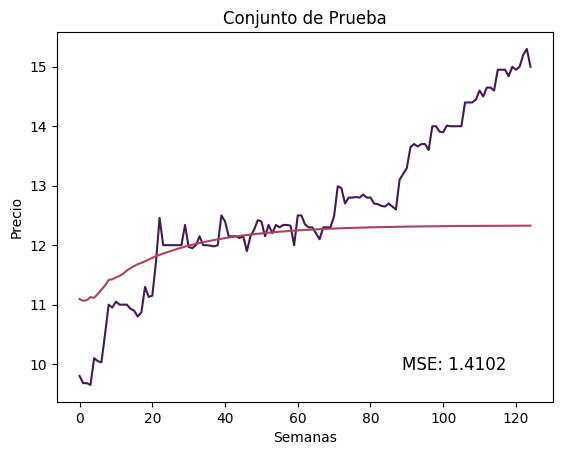
\includegraphics[width=\linewidth]{Figuras/proceso_de_entrenamiento/grafs_c_prueba/DWT_LSTM/auto_predictiva/DWT_LSTM_rec.png}
    \end{minipage}
    \caption{Desempeño auto-predictivo de la DWT-LSTMnn en conjunto de prueba: muestreo aleatorio y temporal.} 
    \label{fig:c_prueba_DWTLSTM_autopred_v2}
\end{figure}

Durante las primeras semanas de la predicción, pareciera que LSTMnn y DWTLSTMnn siguen cierta tendencia de los datos originales, digamos unas diez semanas en el futuro. A pesar de esto vemos que ni las RNNs son capaces de mantener por tanto tiempo el pronóstico. Sin embargo, comparado con los modelos auto-regresivos, mejora notablemente al no usar siquiera la técnica FD.

\newpage

\subsection{GRUnn}

De la misma manera y parámetros que la LSTMnn:

\begin{figure}[H]
    \begin{minipage}{0.5\textwidth}
        \centering
        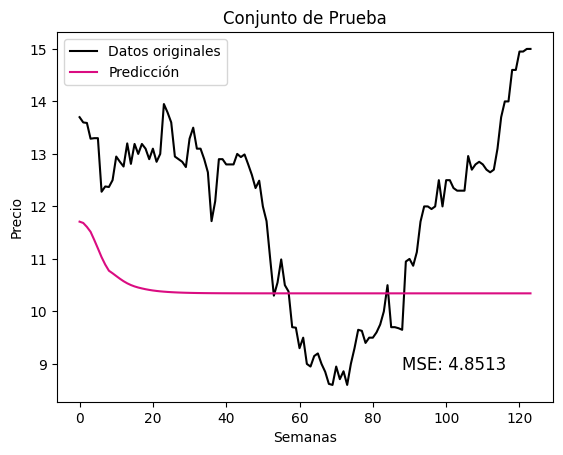
\includegraphics[width=\linewidth]{Figuras/proceso_de_entrenamiento/grafs_c_prueba/muestreo_aleatorio/GRU/auto_predictiva/GRU.png}
    \end{minipage}
    \begin{minipage}{0.5\textwidth}
        \centering
        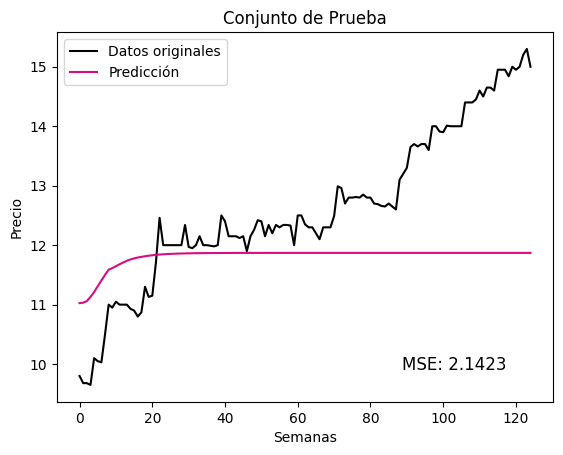
\includegraphics[width=\linewidth]{Figuras/proceso_de_entrenamiento/grafs_c_prueba/GRU/auto_predictiva/GRU.png}
    \end{minipage}
    \caption{Desempeño auto-predictivo de la GRUnn en conjunto de prueba.} 
    \label{fig:c_prueba_GRU_autopred}
\end{figure}

%\newpage

\subsection{DWT-GRUnn}

De la misma manera y parámetros que la DWT-LSTMnn:

\begin{figure}[H]
    \centering
    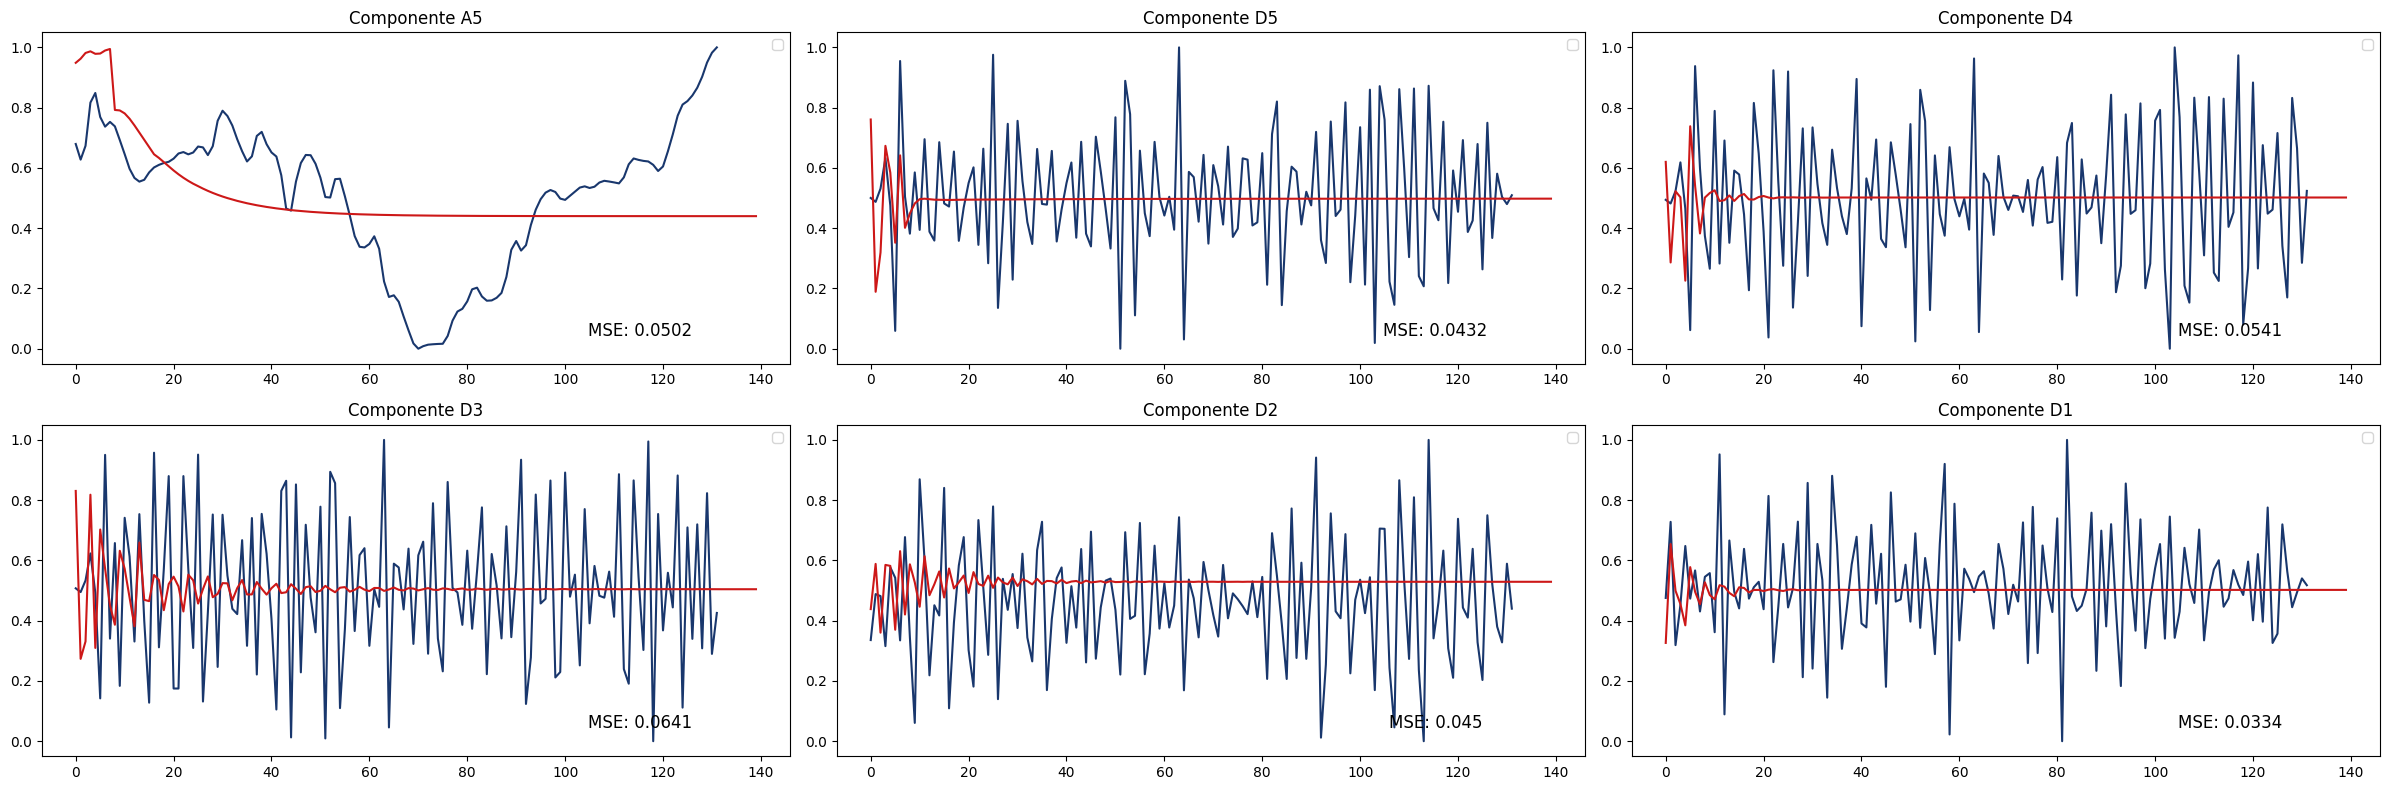
\includegraphics[width=0.9\textwidth]{Figuras/proceso_de_entrenamiento/grafs_c_prueba/muestreo_aleatorio/DWT_GRU/auto_predictiva/DWT_GRU.png}
    \caption{Predicciones auto-predictivas de la DWT-GRUnn de los componentes del conjunto de pruebas de muestro aleatorio.} 
    \label{fig:c_prueba_componentes_DWTGRU_autopred_muestreo_aleatorio}
\end{figure}

\begin{figure}[H]
    \centering
    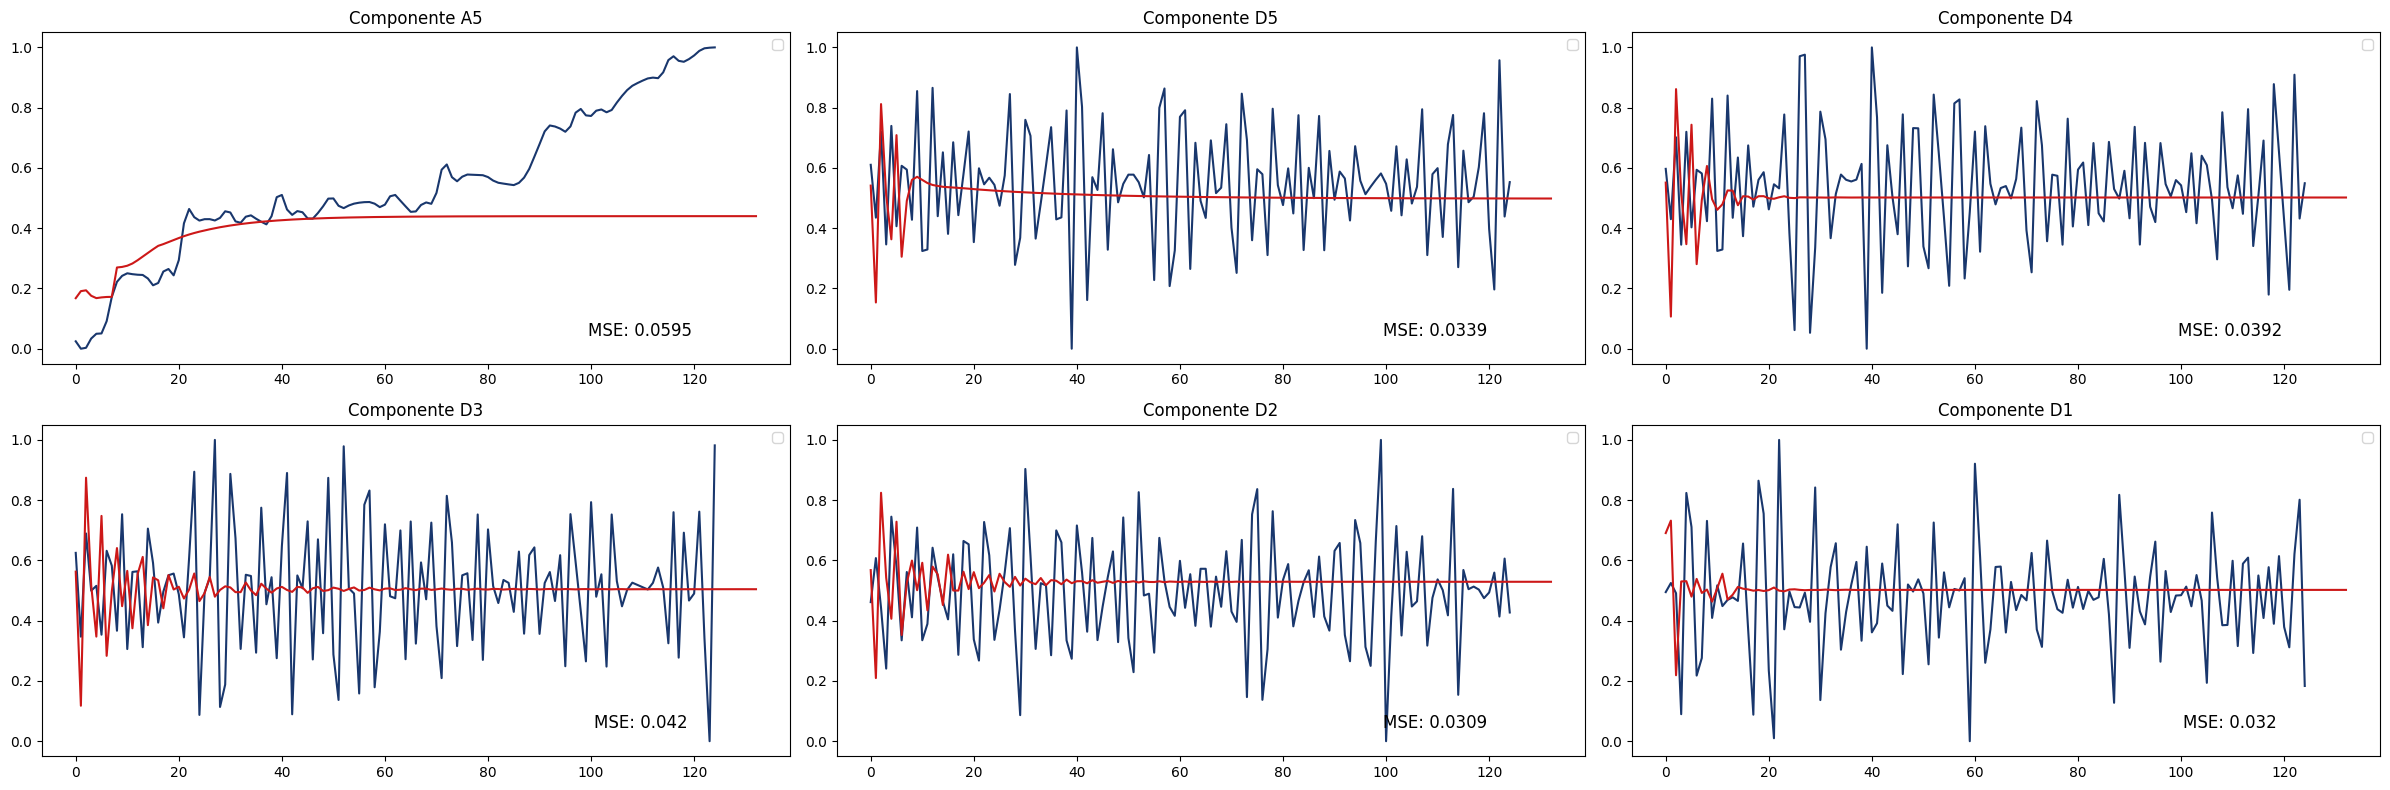
\includegraphics[width=0.9\textwidth]{Figuras/proceso_de_entrenamiento/grafs_c_prueba/DWT_GRU/auto_predictiva/DWT_GRU.png}
    \caption{Predicciones auto-predictivas de la DWT-LSTMnn de los componentes del conjunto de pruebas de muestro temporal.} 
    \label{fig:c_prueba_componentes_DWTGRU_autopred}
\end{figure}

\begin{figure}[H]
    \begin{minipage}{0.5\textwidth}
        \centering
        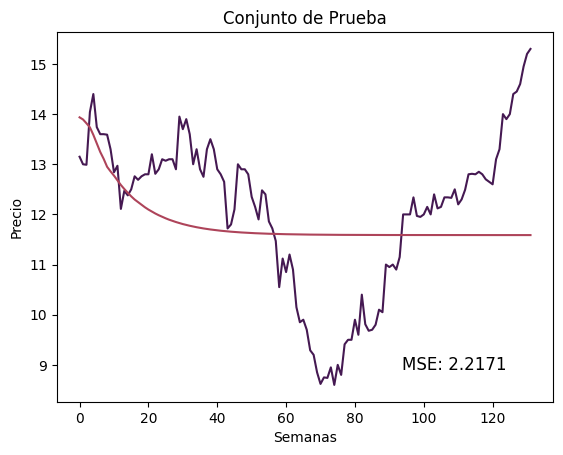
\includegraphics[width=\linewidth]{Figuras/proceso_de_entrenamiento/grafs_c_prueba/muestreo_aleatorio/DWT_GRU/auto_predictiva/DWT_GRU_rec.png}
    \end{minipage}
    \begin{minipage}{0.5\textwidth}
        \centering
        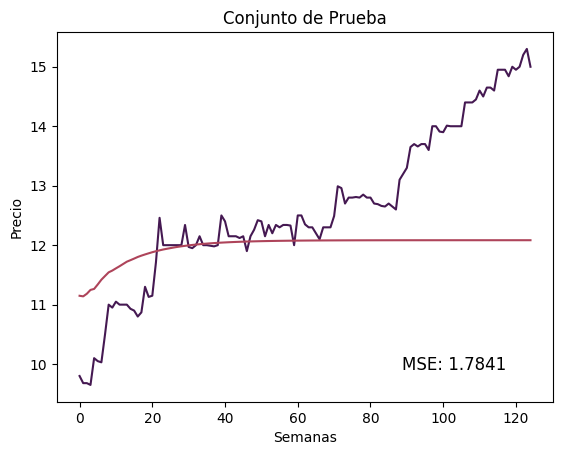
\includegraphics[width=\linewidth]{Figuras/proceso_de_entrenamiento/grafs_c_prueba/DWT_GRU/auto_predictiva/DWT_GRU_rec.png}
    \end{minipage}
    \caption{Desempeño auto-predictivo de la DWT-GRUnn en conjunto de prueba: muestreo aleatorio y temporal.} 
    \label{fig:c_prueba_DWTGRU_autopred_v2}
\end{figure}

Como se vió, los modelos no son aptos para este tipo de escenarios, pero los que han sido mejor evaluados, al menos durante las primeras semanas del análisis son sin duda los recurrentes.